\usepackage{wasysym}\documentclass[12pt,a4paper,titlepage,listof=totoc,bibliography=totoc,chapteratlists=0pt]{scrreprt}

\begin{filecontents*}{\jobname.xmpdata}
	\Keywords{VR, IOT, TODO}
	\Title{Unser tolles Thema -- wir sind suppa}
	\Author{Stefan Schwammal, Susi Schwammal}
\end{filecontents*}

\setcounter{tocdepth}{1}

\usepackage[utf8]{inputenc}
\usepackage[T1]{fontenc}
\usepackage{amsmath}
\usepackage{amsfonts}
\usepackage{amssymb}
\usepackage[table]{xcolor}
\usepackage{graphicx}
\usepackage[left=3.50cm, right=2.00cm, top=2.00cm, bottom=2.00cm,foot=1cm]{geometry}
\usepackage[splitrule,hang,flushmargin,multiple,bottom]{footmisc}
\usepackage{lmodern, textcomp}
\usepackage{lmodern}
\usepackage{pdfpages}
\usepackage[ngerman]{babel}
\usepackage{multicol}
\usepackage{subfig}
\usepackage{float}
\usepackage{array,tabularx,booktabs}
\usepackage{ragged2e}
\usepackage{lipsum}
\usepackage{wrapfig}

\newcolumntype{M}[1]{>{\centering\arraybackslash}m{#1}}

\usepackage{enumitem}
\newlist{compactitem}{itemize}{3}
\setlist[compactitem,1]{label=\textbullet, nosep,leftmargin=1.5em,labelwidth=*,align=left}
\setlist[compactitem,2]{label=--, nosep,leftmargin=1.5em,labelwidth=*,align=left}
\setlist[compactitem,3]{label=\textopenbullet, nosep,leftmargin=1.5em,labelwidth=*,align=left}
\newlist{compactenum}{enumerate}{3}
\setlist[compactenum,1]{label=\arabic*., nosep,leftmargin=1.5em,labelwidth=*,align=left}
\setlist[compactenum,2]{label=\alph*., nosep,leftmargin=1.5em,labelwidth=*,align=left}
\setlist[compactenum,3]{label=\roman*., nosep,leftmargin=1.5em,labelwidth=*,align=left}
\newlist{compactdesc}{description}{3}
\setlist[compactdesc]{leftmargin=1.5em,labelwidth=*,align=left}

\usepackage{microtype}

\usepackage[parfill]{parskip}

\definecolor{bluekeywords}{rgb}{0.13,0.13,1}
\definecolor{greencomments}{rgb}{0,0.5,0}
\definecolor{redstrings}{rgb}{0.9,0,0}
\definecolor{lightgray}{gray}{0.9}
\definecolor{lightblue}{rgb}{0.93,0.95,1.0}

\usepackage{listings}

\makeatletter
\lstdefinestyle{lststyle}{
	basicstyle=%
	\ttfamily
	\lst@ifdisplaystyle\scriptsize\fi
}
\makeatother

\renewcommand{\lstlistlistingname}{List of Listings}
% TODO: define other languages as needed
\lstset{language=Python,
numbers=left,               
numberstyle=\tiny,          
showspaces=false,
showtabs=false,
breaklines=true,
lineskip=-1pt,
tabsize=2,
showstringspaces=false,
breakatwhitespace=true,
escapeinside={(*@}{@*)},
commentstyle=\color{greencomments},
keywordstyle=\color{bluekeywords}\bfseries,
stringstyle=\color{redstrings},
style=lststyle,
xleftmargin=17pt,
         framexleftmargin=17pt,
         framexrightmargin=5pt,
         framexbottommargin=4pt
}
\lstset{
morekeywords={base,var,in,out,dynamic,from,where,select,orderby,function,\$,group,by,into,yield,async,await,@,None,self,as,elif,with}
}
\lstdefinelanguage{TypeScript}{
	keywords={typeof, new, true, false, catch, function, return, null, switch, var, if, in, while, do, else, case, break, void, number, string, boolean, module, \$, export, for, this},
	keywordstyle=\color{blue}\bfseries,
	ndkeywords={class, export, boolean, throw, implements, import, this},
	ndkeywordstyle=\color{darkgray}\bfseries,
	identifierstyle=\color{black},
	sensitive=false,
	comment=[l]{//},
	morecomment=[s]{/*}{*/},
	commentstyle=\color{purple}\ttfamily,
	stringstyle=\color{red}\ttfamily,
	morestring=[b]',
	morestring=[b]"
}
\usepackage{caption}
\DeclareCaptionFont{white}{\color{white}}
\DeclareCaptionFormat{listing}{\colorbox[cmyk]{0.43, 0.35, 0.35,0.01}{\parbox{\textwidth}{\hspace{10pt}#1#2#3}}}
\captionsetup[lstlisting]{format=listing,labelfont=white,textfont=white} 
\captionsetup[table]{justification=centering, singlelinecheck=false}

\usepackage{setspace}
\newcommand{\MSonehalfspacing}{%
	\setstretch{1.44}%  default
	\ifcase \@ptsize \relax % 10pt
	\setstretch {1.448}%
	\or % 11pt
	\setstretch {1.399}%
	\or % 12pt
	\setstretch {1.433}%
	\fi
}

\newcommand{\setauthor}[1]{\ohead[]{#1}}

\usepackage[automark]{scrlayer-scrpage}
\pagestyle{scrheadings}
\automark{chapter}
\renewcommand\sectionmark[1]{\markright{\MakeMarkcase {\thesection\hskip .5em\relax#1}}}
\rohead{\ifnum\expandafter\pdfstrcmp\botmark=0 \rightmark\else\leftmark{} --- \rightmark\fi}
\ihead[]{\headmark}
\chead[]{}
\ohead{}
\cfoot[]{}
\ofoot[\pagemark]{\pagemark}
\setheadsepline{.1pt}

\usepackage[hyphens]{url}

\usepackage[a-1b]{pdfx}

\usepackage{hyperref}
\hypersetup{pdfa}

\usepackage[nonumberlist,toc,nopostdot]{glossaries}

\usepackage{chngcntr}
\counterwithout{footnote}{chapter}
\counterwithout{figure}{chapter}
\counterwithout{table}{chapter}
\AtBeginDocument{
	\counterwithout{lstlisting}{chapter}
	\urlstyle{sf}
}
\newcounter{RPages}

\makeatletter
\def\bstctlcite{\@ifnextchar[{\@bstctlcite}{\@bstctlcite[@auxout]}}
\def\@bstctlcite[#1]#2{\@bsphack
	\@for\@citeb:=#2\do{%
		\edef\@citeb{\expandafter\@firstofone\@citeb}%
		\if@filesw\immediate\write\csname #1\endcsname{\string\citation{\@citeb}}\fi}%
	\@esphack}
\makeatother

\clubpenalty=10000
\widowpenalty=10000
\displaywidowpenalty=10000
\interfootnotelinepenalty=10000

\title{Leobot - Chatbot für die HTL Leonding}
\author{Felix Dumfarth, Lukas Starka}

\makeindex
\makeglossaries
\begin{document}
\bstctlcite{IEEEexample:BSTcontrol}
\newcommand{\reminder}[1]
{ \textcolor{red}{<[{\bf\marginpar{\mbox{$<==$}} #1 }]>} }
\newcommand{\icode}[1]{\lstinline$#1$}
%\urlstyle{same}
%\setstretch{1.5}
\setstretch {1.433}
\renewcommand{\arraystretch}{1.2}


\includepdf{./titlepage/coversheet}
\pagenumbering{Roman}
\newpage
\thispagestyle{empty}
\vspace{3cm}
~ \\ \\
Ich erkläre an Eides statt, dass ich die vorliegende Diplomarbeit selbstständig und ohne fremde Hilfe verfasst, andere als die angegebenen Quellen und Hilfsmittel nicht benutzt bzw. die wörtlich oder sinngemäß entnommenen Stellen als solche kenntlich gemacht habe.

Die Arbeit wurde bisher in gleicher oder ähnlicher Weise keiner anderen Prüfungsbehörde vorgelegt und auch noch nicht veröffentlicht.

Die vorliegende Diplomarbeit ist mit dem elektronisch übermittelten Textdokument identisch.
\vspace{3cm}
% Hier kommt die Unterschrift drüber
\begin{tabbing}
Leonding, April 2022 \hspace{5cm} S. Schwammal \& S. Schwammal
\end{tabbing}
\vspace{10cm}
Zur Verbesserung der Lesbarkeit wurde in diesem Dokument auf eine geschlechtsneutrale Ausdrucksweise verzichtet.
Alle verwendeten Formulierungen richten sich jedoch an alle Geschlechter.
\newpage
\setcounter{page}{1}

\begin{spacing}{1}
    \chapter*{Abstract}
\end{spacing}
\begin{wrapfigure}{r}{0.3\textwidth}
    \begin{center}
      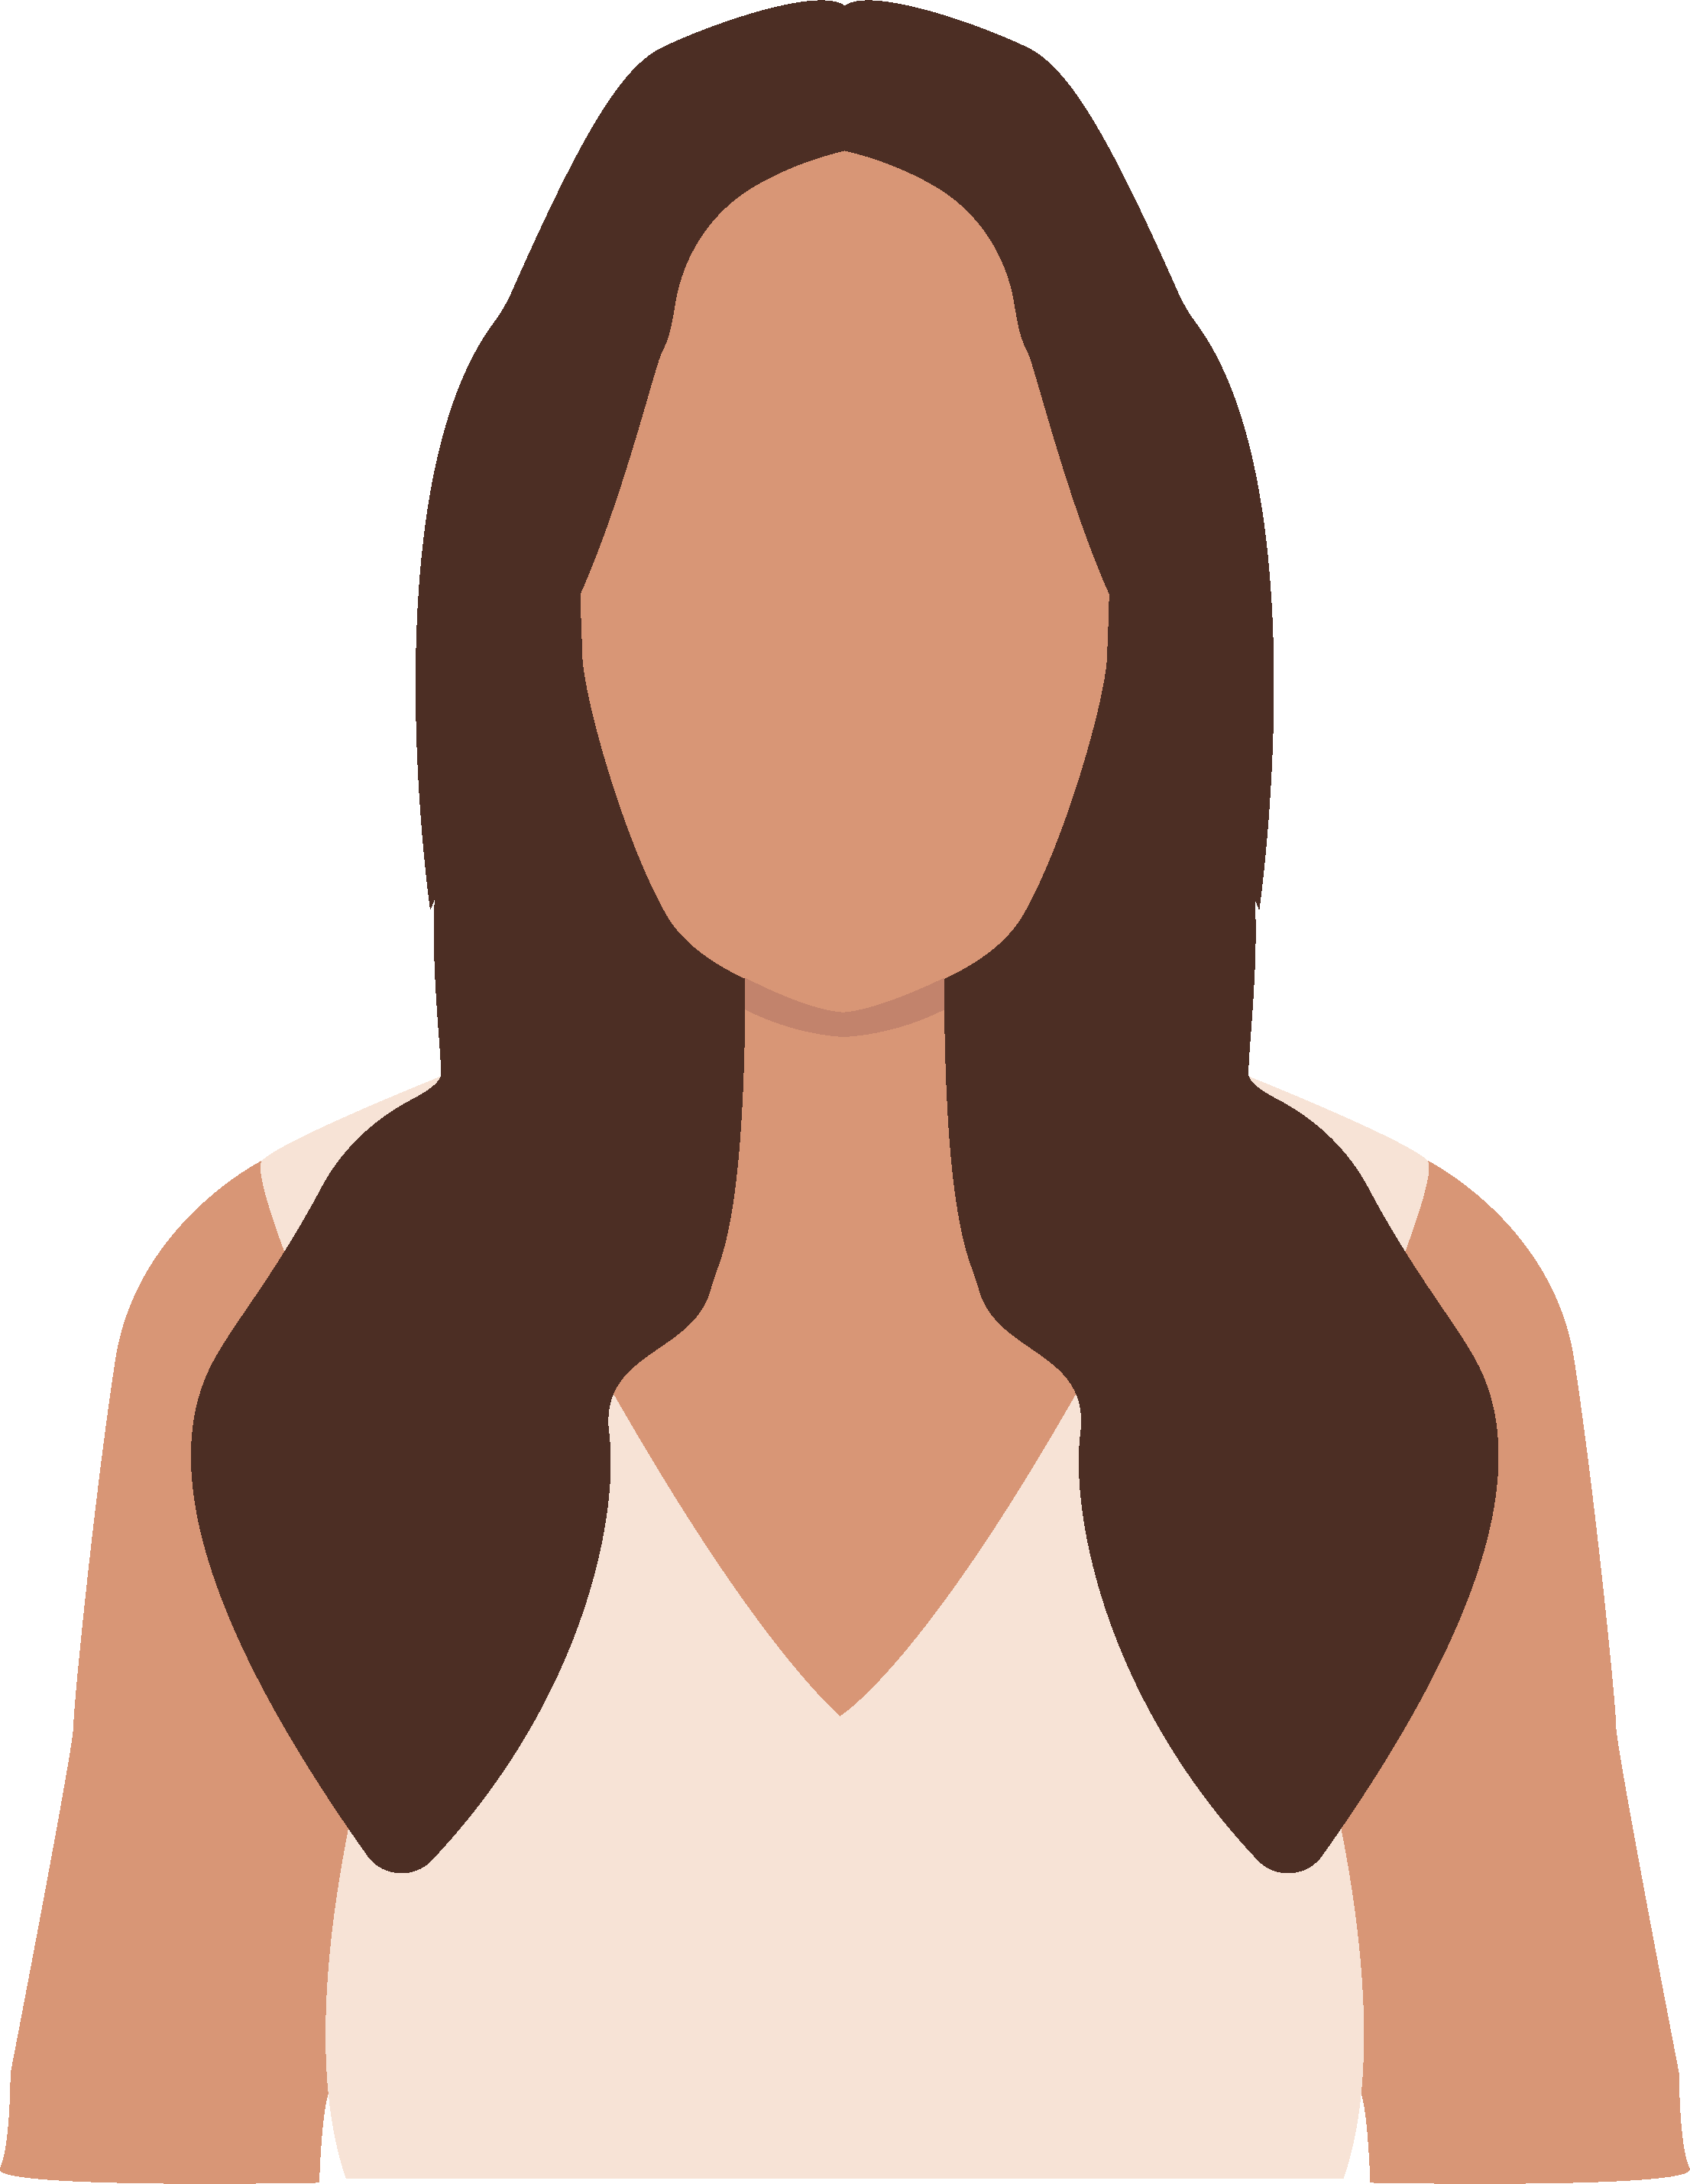
\includegraphics[width=0.2\textwidth]{pics/LeonieTrans.png}
    \end{center}
\end{wrapfigure}
This diploma thesis deals with the topic of a chatbot that was created with the help of Rasa and can be found on the HTL Leonding website. This chatbot should be able to provide interested people with answers about the school quickly and easily, saving visitors from having to search around on the website and calling and asking the secretariat.

\newpage
\begin{spacing}{1}
    \chapter*{Zusammenfassung}
\end{spacing}
\begin{wrapfigure}{r}{0.3\textwidth}
    \begin{center}
      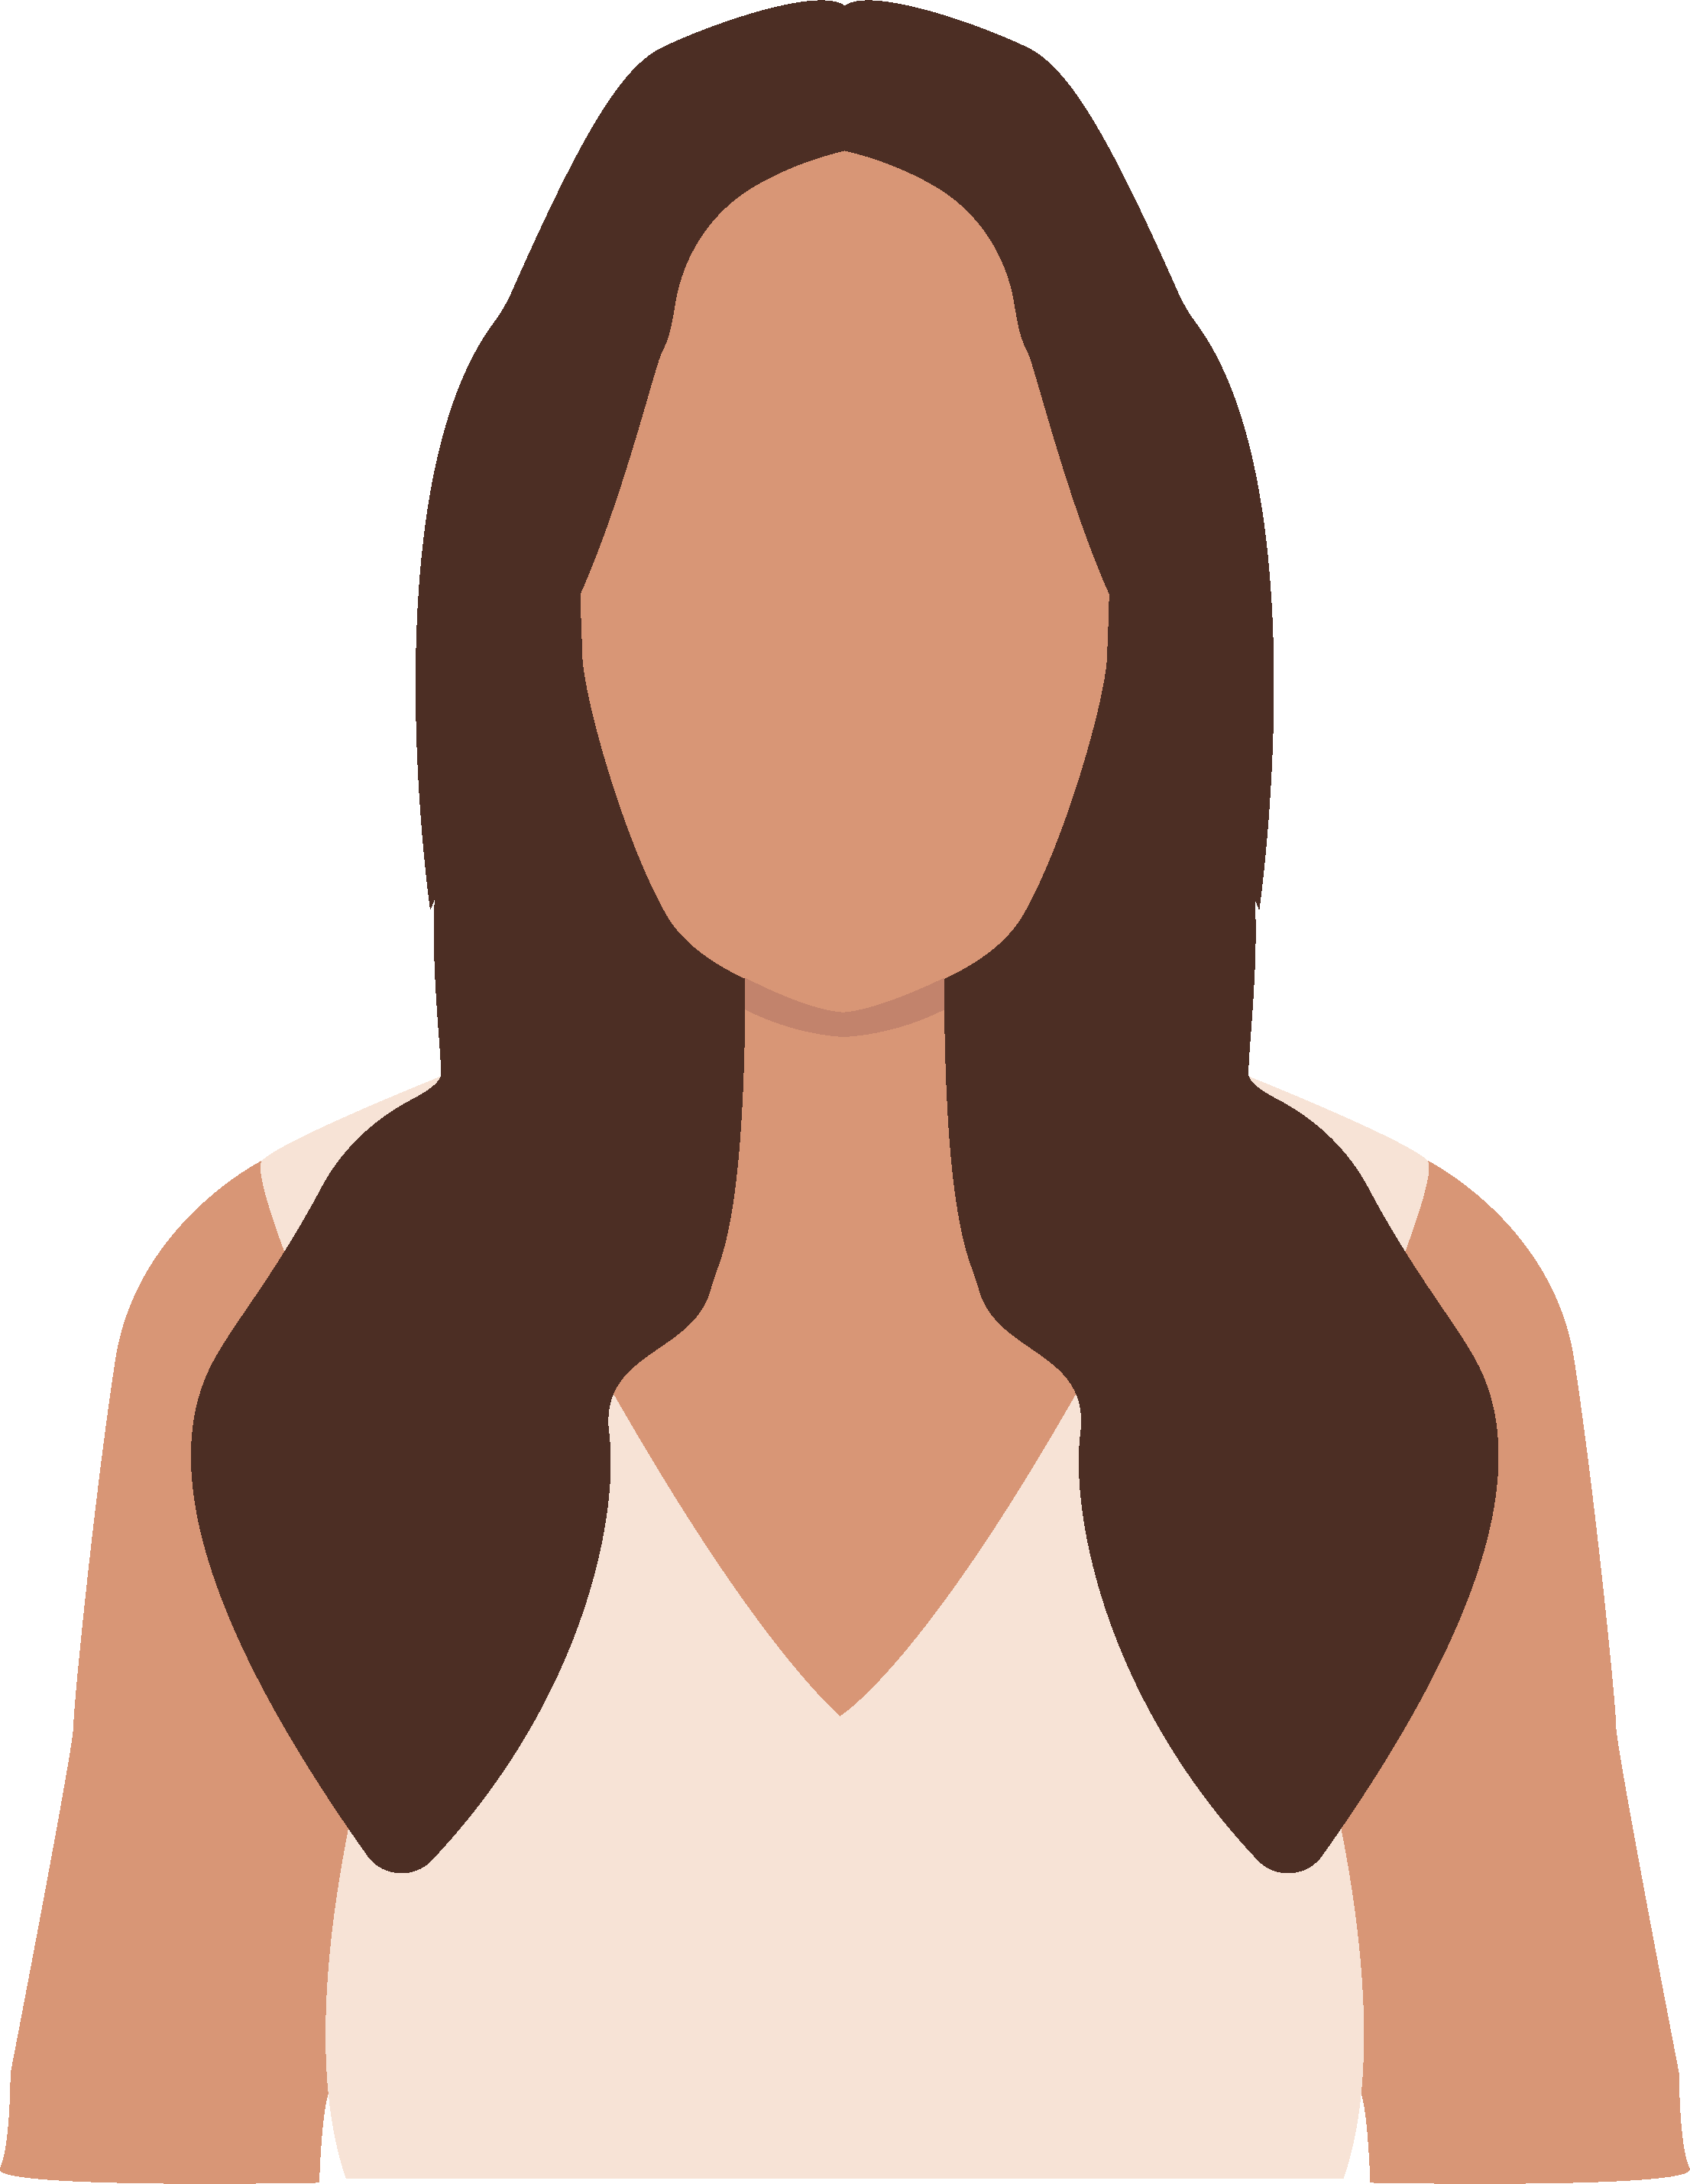
\includegraphics[width=0.2\textwidth]{pics/LeonieTrans.png}
    \end{center}
\end{wrapfigure}
Die vorliegende Diplomarbeit beschäftigt sich mit dem Thema eines Chatbots, der mithilfe von Rasa erstellt worden ist und auf der Webseite der HTL Leonding zu finden sein soll. Dieser Chatbot soll interessierten Person einfach und schnell Antworten über die Schule liefern können und somit den Besuchern ein herumsuchen auf der Webseite sparen sowie anrufe und nachfragen beim Sekritäriat.


\pagestyle{plain}

\renewcommand{\lstlistlistingname}{Quellcodeverzeichnis}

\tableofcontents
\newpage
\setcounter{RPages}{\value{page}}
\setcounter{page}{0}
\pagenumbering{arabic}
\pagestyle{scrheadings}

\begin{spacing}{1}
\chapter{Einleitung}\label{chapter:introduction}
\end{spacing}
\section{Struktur der Diplomarbeit}
Die Folgenden Themengebiete wurden in der Diplomarbeit abgewickelt:

\textbf{Technischer Hintergrund} präsentiert notwendiges Vorabwissen über maschinelles Lernen und damit verbunde Themengebiete wie Deep Learning und neuronale Netze, deren Verständnis relevant für die darauffolgenden Themengebiete ist.

\textbf{Toolstack} präsentiert die verwendeten Tools und Technologien, die zur Erstellung der Diplomarbeit genutzt wurden.

\textbf{Chatbots am Beispiel Rasa} präsentiert die Komponenten und die Entwicklung eines Chatbots mit Rasa ins detail.

\textbf{Implementierung} präsentiert die Entwicklung und Umsetzung des Chatbots und seinen Begleitprodukten aus dem praktischen Teil der Diplomarbeit.

\textbf{Evaluation}



\section{Ausgangslage}
\setauthor{Felix Dumfarth}
Zahlreiche Organisationen bauen heutzutage auf eine starke Webpräsenz und wickeln dabei komplexe Produkt\- oder Leistungsfunktionalitäten ab.
Eine wichtige Rolle spielt dabei nicht nur der Kundenservice, sondern auch die Kommunikation, denn die Nutzer erwarten eine möglichst zeitnahe Beratung.
Die Bereitstellung von solchen Services ist derzeit immer noch mit sehr hohen Kosten verbunden.

\section{Istzustand}
\setauthor{Felix Dumfarth}
Es gibt viele Personen, die sich für die HTL Leonding interessiert sind und sich gerne schnell über die Schule informieren wollen.


\section{Problemstellung}
\setauthor{Felix Dumfarth}
Die HTL Leonding hat ein großes Informationsangebot, zu diesem gibt es viele Zugänge, zum Beispiel auf der Website ist es oft schwierig, den Überblick zu bewahren mit den vielen Unterseiten und daher wäre eine Unterstützung zum Finden für die vielen Informationen hilfreich.

\section{Aufgabenstellung}
\setauthor{Felix Dumfarth}
In dieser vorliegenden Arbeit soll ein Chatbot für die HTL Leonding Website erstellt werden, der Besucherinnen und Besuchern einfach und schnell schulspezifische Fragen beantworten soll.
Jedoch soll es auch möglich sein, dass der Bot auch als Grundlage für weitere Arbeiten in der Schule, wie zum Beispiel der 3-D-Leonie, zum Einsatz kommen kann.

\section{Use-Cases}
\setauthor{Felix Dumfarth}

\begin{figure}[hbt!]
    \centering
    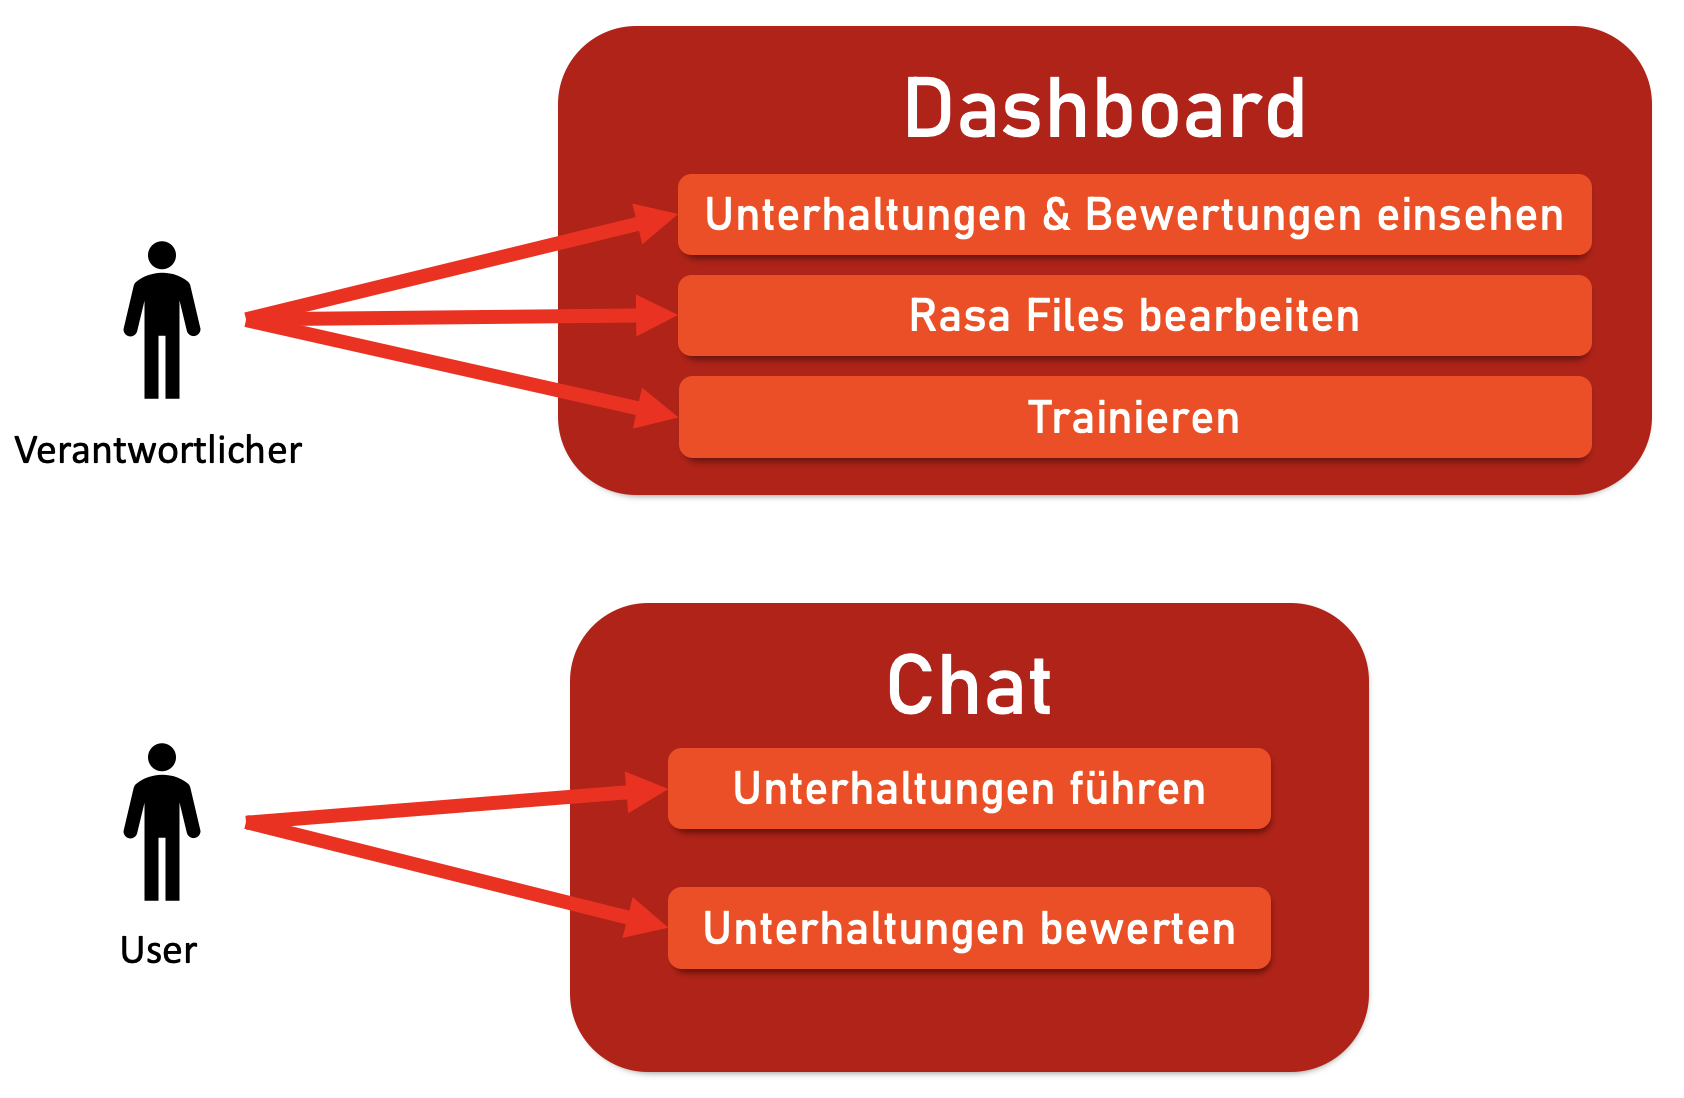
\includegraphics[scale=0.5]{pics/usecase}
    \caption{Use-Case Diagramm}
    \label{fig:impl:usecase}
\end{figure}

Der User kann hauptsächlich schulspezifische Unterhaltungen mit dem Chatbot führen und diese Unterhaltung anhand ihrer Qualität bewerten.
Eine verantwortliche Person kann sich die Unterhaltungen und Bewertungen von Usern ansehen, sodass diese beurteilt werden können.
Außerdem kann die verantwortliche Person die Rasa Files \texttt{nlu.yml}, \texttt{stories.yml}, \texttt{rules.yml} und \texttt{domain.yml} bearbeiten und den Chatbot auffordern, sein neu erlerntes Wissen einzutrainieren.


\begin{spacing}{1}
\chapter{Technischer Hintergrund}
\end{spacing}
\section{Maschinelles Lernen}
\setauthor{Lukas Starka}


\section{Deep Learning}
\setauthor{Lukas Starka}


\section{Neuronale Netze}
\setauthor{Lukas Starka}
\subsection{Convolutional Neural Networks}
\setauthor{Lukas Starka}

\subsection{Recurrent Neural Networks}
\setauthor{Lukas Starka}


\section{Word Vectors}
\setauthor{Lukas Starka}


\section{Text Analysis}
\setauthor{Lukas Starka}

\subsection{Text analysis vs. Text Mining vs. Text Analytics}
\setauthor{Lukas Starka}

Meistens werden die Begriffe Text Analysis und Text Mining im selben Zusammenhang verwendet.
Dabei bedeuten sie eigentlich dasselbe, nämlich, dass man den Sinn einer Nachricht extrahiert.
Deswegen wird in den folgenden Kapiteln nur von Text Analysis gesprochen.

Es gibt jedoch einen Unterschied zwischen Text Analysis und Text Analytics.
Grundsätzlich kann man dabei sagen, dass Text Analysis qualitative Ergebnisse liefert, wohingegen bei Text Analytics die Quantität mehr im Vordergrund steht.\cite{textAnalysisMonkeylearn, machineLearningTextAnalysis}

Bei Text Analysis werden also wichtige Informationen aus der Nachricht herausgelesen.
Oder anders formuliert geht es darum, dass trotz der Vielseitigkeiten der menschlichen Sprache trotzdem die Kernaussage herausgefunden werden kann, mit der dann gearbeitet wird.
Es können also dann Informationen herausgefiltert werden, wie beispielsweise, ob etwas positiv oder negativ ist oder was das Hauptthema des Textes ist.\cite{textAnalysisMonkeylearn, machineLearningTextAnalysis}

Auf der anderen Seite wird bei Text Analytics werden verschiedene Muster aus einer großen Menge an Nachrichten herausgefiltert, welche dann in Graphen, Tabellen oder Berichten gezeigt werden können.
Bei Text Analytics geht es also darum Muster und Entwicklungen von numerischen Ergebnissen herauszufinden, bei denen dann Informationen herausgefiltert werden können, wie beispielsweise, die Prozentzahl der positiven Bewertungen.\cite{textAnalysisMonkeylearn, machineLearningTextAnalysis}

\subsection{Warum Text Analysis?}
\setauthor{Lukas Starka}

Im Gegensatz zum manuellen Aufbereiten von Texten sorgt Machine Learning für eine schnelle Bearbeitung, die außerdem auch kostengünstiger ist, weil viele Stellen wegfallen, die benötigt werden würden, um die Texte selber aufzubereiten.
Durch die Verwendung von Text Analysis spart man sich viele Arbeitskräfte, die bei anderen wichtigen Aufgaben innerhalb eines Unternehmens eingesetzt werden können.
Außerdem können dadurch Texte rund um die Uhr und zur Echtzeit bearbeitet werden.
Durch Algorithmen werden außerdem Fehler reduziert, die bei manuellem Bearbeiten leicht auftreten können und Daten können genauer aufbereitet werden.\cite{textAnalysisMonkeylearn}

\subsection{Machine Learning mit Text Analysis}
\setauthor{Lukas Starka}

Grob kann man behaupten, dass ein Text Analysis Tool aus drei verschiedenen Schritten besteht.

\begin{enumerate}
    \item Zunächst muss man sich überlegen, welche Daten gesammelt werden sollen, um damit sein Modell zu trainieren und zu testen.
    Man unterscheidet hierbei zwischen "Internal Data" und "External Data".
    Unter External Data werden Quellen, wie Zeitungen oder Foren bezeichnet und zu der Internal Data zählen sämtliche Daten, die eine Firma jeden Tag generiert, wie E-Mails, Reports, Chats oder Umfragen.
    \item Danach müssen die Daten vorbereitet werden, damit das Programm diese versteht.
    Dieser Schritt wird meistens als "Data Preprocessing" bezeichnet.
    \item Zum Schluss wird dann ein Machine Learning Algorithmus hinzugefügt, welcher sich um die Analyse kümmert.
    Diesen kann man entweder komplett selber implementieren oder man nimmt sich Libraries zur Hilfe.\cite{machineLearningTextAnalysis}
\end{enumerate}

\section{Natural Language Processing (NLP)}
\setauthor{Lukas Starka}

Natural Language Processing, oft auch als Akronym \textbf{NLP} abgekürzt, sorgt dafür, dass Computer Text auf dieselbe Art und Weise verstehen, wie wir es als Menschen tun.
NLP vereint dabei die Modellierung der menschlichen Sprache mit statistischen Machine Learning und Deep Learning Modellen.
Dies ermöglicht der Maschine im Endeffekt, dass diese menschliche Sprache in Form von Text- oder Sprachdaten zu verarbeiten und sozusagen die komplette Bedeutung und Absicht der Benutzerin oder des Benutzers zu verstehen.\cite{naturalLanguageProcessingIBM}

\subsection{Corpus}
\setauthor{Lukas Starka}

Unter dem Corpus werden die Daten bezeichnet, die verwendet werden, um das NLP Modell zu trainieren, damit dieses menschliche Sprache versteht und damit arbeiten kann.
Der Textkorpus ist also eine Menge von strukturierten Texten, die für den Computer lesbar sind.\cite{corpus}


\subsection{Tokenization}
\setauthor{Lukas Starka}

Bei der Tokenization repräsentiert jeder Token eine sinnvolle Einheit.
Darunter versteht man Wörter, Zeichen oder Sonderzeichen, die alle einen eigenen Token darstellen, lediglich Leerzeichen in einem Satz stellen keine eigenen Token dar.\cite{machineLearningTextAnalysis, naturalLanguageProcessing}

Die verschiedenen Token, die dabei entstehen, können dabei wie folgt aussehen:

\begin{lstlisting}[label={lst: Tokenization}]
Let us go to the park.

0: Let
1: us
2: go
3: to
4: the
5: park
6: .
\end{lstlisting}

Die Tokenization ist dabei besonders für verschiedene Sprachen von Vorteil, da es in diesen immer andere Regeln gibt, wie die Wörter aufgeteilt werden können.
In dem obigen Beispiel wirkt es womöglich no so, als könnte man mit einer \textbf{split()} Methode das selbe Resultat erzielen, aber es gibt auch Besonderheiten einer Sprache, die vom Tokenizer bedacht werden müssen, wie folgendes Beispiel aufzeigt.\cite{machineLearningTextAnalysis, naturalLanguageProcessing}

\begin{lstlisting}[label={lst: Tokenization Ausnahme}]
"Let's go to the U.K.!"

0: "
1: Let
2: 's
3: go
4: to
5: the
6: U.K.
7: !
8: "
\end{lstlisting}

\subsection{Part-of-speech-Tagging (POS-Tagging)}
\setauthor{Lukas Starka}

Beim Part-of-speech-Tagging geht es um das Taggen von Wörtern und deren zugehörigen Teil der Sprache.
Als Teil einer Sprache, also dem Part-of-speech, werden grundsätzlich Wörter bezeichnet, die ähnliche grammatikalische Eigenschaften oder Nutzungen besitzen.
Im deutschen sind hierbei also die verschiedenen Wortarten gemeint.

Beim Tagging werden entweder Statistiken angewendet, wie beispielsweise, dass es sehr wahrscheinlich ist, dass nach einem Artikel ein Nomen folgt.
Außerdem gibt es sogenannte Rule-Based POS-Taggers, deren Aufgabe es ist, vordefinierte Regeln zu verwenden, um das Tagging zu vollziehen.\cite{machineLearningTextAnalysis, naturalLanguageProcessing}

Ein Beispiel für POS-Tagging könnte also folgendermaßen aussehen:

\begin{lstlisting}[label={lst: POS-Tagging}]
I am going to the U.K.

I: Pronoun
am: Verb
going: Verb
to: Part
the: Article
U.K.: Noun
\end{lstlisting}

\subsection{Named-entity recognition (NER)}
\setauthor{Lukas Starka}

Named-entity recognition ist eine der wichtigsten Säulen von Natural Language Processing.
Entities sind strukturierte Stücke von Informationen, die sich innerhalb der Nachricht einer Benutzerin oder eines Benutzers befinden.
Dabei werden Entities aus Texten erkannt und anschließend mit einem Tag der zugehörigen Kategorie versehen.\cite{namedEntityRecognition}

Beispiele für Entities wären also:

\begin{lstlisting}[label={lst: NER-Tagging}]
PERSON      Personen (inklusive fiktionalen Personen)
NORP        Nationalitäten oder religiöse oder politische Gruppen
FACILITY    Gebäude, Flughäfen, Brücken, Straßen
LOC         Orte
PRODUCT     Objekte, Fahrzeuge, Essen
LANGUAGE    Sprachen
\end{lstlisting}

\subsection{Stemming}
\setauthor{Lukas Starka}

Beim Preprocessing von Texten sind außerdem das Stemming und die Lemmatization Schritte, die häufig durchgeführt werden.

Beim Stemming wird der Wortstamm eines Tokens von den Präfixen und Suffixen gelöst.
Unter einem Präfix versteht man eine Vorsilbe, die dem Wortstamm vorangestellt wird und bei dem Suffix, handelt es sich im Gegenzug dazu um Worterweiterungen, die dem Stamm folgen.
Hierbei gibt es wieder die Möglichkeit selber einen Stemmer zu implementieren oder bereits vorgefertigte Stemmer zu verwenden.\cite{textAnalysisMonkeylearn, machineLearningTextAnalysis}

Ein Beispiel für Stemming wäre also wie folgt:

\begin{lstlisting}[label={lst: Stemming}]
Buying ---> buy

unpredictability ---> un + predict + able + ity
un          prefix
predict     base word
able        suffix
ity         suffix
\end{lstlisting}

\subsection{Lemmatization}
\setauthor{Lukas Starka}

Unter der Lemmatization oder auch Lemmatisierung wird der Prozess verstanden, bei dem alle verschiedenen Arten von einem Wort zu ihrem Wortstamm umgeformt werden.

Die Lemmatisierung ist sozusagen eine Weiterentwicklung des Stemming und versucht im Gegensatz zum Stemming den Kontext zu den Wörtern zu bringen.
Je nachdem in welchem Kontext die Verben gebraucht werden können sie sich dabei von ihrer Wortart unterscheiden und so eine andere Bedeutung haben.
Generell lässt sich sagen, dass Stemmer meist einfacher zu implementieren sind und für schnellere Laufzeiten sorgen, allerdings wird von vielen auch die Lemmatization dem Stemming vorgezogen, aufgrund der Vorteile die das Einbeziehen des Kontextes mit sich bringt.\cite{machineLearningTextAnalysis, textAnalysisMonkeylearn, stemmingLemmatization, }


Beispiele für die Lemmatisierung sind:

\begin{lstlisting}[label={lst: Lemmatization}]
better ---> good
walking ---> walk
walked ---> walk
walks ---> walk
meeting ---> meet (wenn es als Verb gebraucht wird)
\end{lstlisting}

\subsection{Parsing}
\setauthor{Lukas Starka}

Parsing könnte man so beschreiben, dass es eine Art ist um einen Satz auseinanderzuteilen, um die Struktur des Satzes besser zu verstehen.
Beim Parsing wird also die syntaktische Struktur eines Textes bestimmt.
Um dies zu erreichen, nimmt der Parsing Algorithmus die Eigenheiten der Grammatik, von der jeweiligen Sprache, in der der Text geschrieben ist, her.\cite{textAnalysisMonkeylearn}

Es gibt zwei verschiedene Arten von Parsing.
Diese sind das sogenannte "Dependency Parsing" und das sogenannte "Constituency Parsing".

\subsubsection{Dependency Parsing}
\setauthor{Lukas Starka}

Beim Dependency Parsing wird die grammatische Struktur eines Satzes bestimmt.
Außerdem kann man mithilfe des Dependency Parsing herausfinden, welche Wörter zusammenhängen und welche Beziehung diese zueinander aufweisen.
Dies bedeutet beispielsweise, dass man bei den Wörtern "blauer Ball", "nette Frau" oder ähnlichem erkennen kann, dass sich die Wörter "blau" oder "nett" auf das nachfolgende Wort bezieht.
Ein anderes Beispiel könnten die Wörter "black" und "car" sein.

\begin{figure}[hbt!]
    \centering
    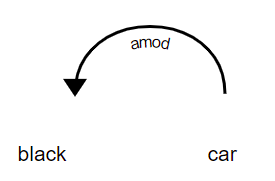
\includegraphics[scale=1]{pics/dependency_parsing}
    \caption{Beispiel für die Beziehung zweier Wörter beim Dependency Parsing~\cite{dependencyParsing}}
    \label{fig:dependency_parsing_relation}
\end{figure}

Wie man dieser Grafik entnehmen kann, bezieht sich die Farbe Schwarz in diesem Fall auf das Auto.
Im Englischen wird das Wort "car" deswegen auch als "Head" bezeichnet und "black" ist ein "child", also ein Wort, dass abhängig von diesem "Head" ist.
Die Beziehung, die zwischen diesen Wörtern vorliegt, wird mit "amod" bezeichnet.
Dies ist eine Abkürzung für "Adjectival Modifier", also ein Adjektiv, welches ein Nomen modifiziert und zu der Bedeutung des Nomens beiträgt.
In diesem Fall gibt dieses eine genaue Beschreibung der Farbe des Autos.\cite{dependencyParsing}

Diese Beziehungen kann man auch in einem Tree darstellen.

\begin{figure}[hbt!]
    \centering
    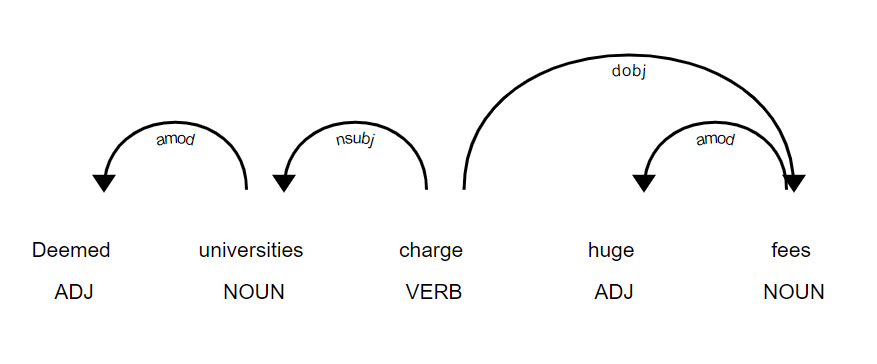
\includegraphics[scale=0.5]{pics/dependency_parsing_tree}
    \caption{Darstellung des Dependency Parsing~\cite{dependencyParsing}}
    \label{fig:dependency_parsing_tree}
\end{figure}

\subsubsection{Constituency Parsing}
\setauthor{Lukas Starka}


\subsection{Stopwords}
\setauthor{Lukas Starka}


\subsection{Vectorization}
\setauthor{Lukas Starka}


\subsection{Skalarprodukt}
\setauthor{Lukas Starka}

\subsection{Kreuzprodukt}
\setauthor{Lukas Starka}


\subsection{Bag of Words}
\setauthor{Lukas Starka}


\subsection{Bag of n-grams}
\setauthor{Lukas Starka}


\subsection{Vector Spaces}
\setauthor{Lukas Starka}


\subsection{Term Frequency times Inverse Document Frequency (TF-IDF)}
\setauthor{Lukas Starka}


\subsection{Zipfsches Gesetz}
\setauthor{Lukas Starka}


\subsection{Word2Vec}
\setauthor{Lukas Starka}


\subsection{NLP und NLU Tools}
\setauthor{Lukas Starka}

Ein paar Beispiele für berühmte Tools, die man nützen kann für Natural Language Understanding (NLU) und Natural Language Processing (NLP) sind:

\begin{itemize}
    \item \href{https://www.nltk.org/}{NLTK}: Das Natural Language Toolkit (kurz NLTK) ist wahrscheinlich die berühmteste Python Library für NLP. NLTK besitzt über 50 Ressourcen für das Bearbeiten von Corpora.
    Außerdem gibt es viele eingebaute Libraries für das Analysieren eines Textes, wie die Klassifikation, Tokenization, Stemming, Tagging, Parsing und Semantic Reasoning.
    \item \href{https://spacy.io/}{SpaCy}: SpaCy ist ebenfalls eine sehr berühmte Bibliothek für Python.
    SpaCy beschreibt sich selbst als "Industrial-Strength Natural Language Processing" und unterstützt über 64 Sprachen.
    SpaCy hat nur einen POS-Tagging-Algorithmus und pro Sprache nur einen Named-Entity-Recognizer, was den Vorteil hat, dass es nicht voller unnötiger Features ist und sich nur auf ein paar wichtige Funktionalitäten konzentriert.
    \item \href{https://www.tensorflow.org/}{TensorFlow}: TensorFlow wird von Google betrieben und ist bei weitem die meist verwendete Library für Deep Learning.
    Außerdem ist die Plattform Open-Source.
    \item \href{https://keras.io/}{Keras}: Keras ist eine Deep Learning Plattform, die in Python geschrieben ist.
    Sie wurde entworfen um schnelle Iterationen und schnelles Ausprobieren mit deep neural networks zu ermöglichen.
    Außerdem bietet Keras ein Interface zu deep neural networks an, welche dann beispielsweise auf TensorFlow, Theano oder anderen Backends laufen können.
    \item \href{https://stanfordnlp.github.io/CoreNLP/}{CoreNLP}: Das CoreNLP Projekt von Stanford ist ein NLP toolkit, welches zwar in Java geschrieben wurde aber auch in anderen Sprachen verwendet werden kann, die auf der JVM Plattform sind.
    \item \href{https://radimrehurek.com/gensim/}{Gensim}: Gensim ist eine Open-Source Library für Python, mit der man semantische NLP Modelle trainieren kann.
    Außerdem ist Gensim Plattform unabhängig und läuft auf jedem Betriebssystem.
    \item \href{https://textblob.readthedocs.io/en/dev/}{TextBlob}: TextBlob ist eine Python Library für das Bearbeiten von Texten.
    \item \href{https://fasttext.cc/}{FastText}: FastText ist eine Open-Source Library, die es Benutzern erlaubt text representations und text classifier zu verwenden.
\end{itemize}


\subsection{NLP in Rasa}
\setauthor{Lukas Starka}

In Rasa kann man sich die verschiedenen Schritte vom Natural Language Processing ansehen, indem man sich die \hyperref[sec:pipeline]{Pipeline} ansieht.
Diese befindet sich in der \textbf{config.yml} Datei und dort sind alle Komponenten aufgelistet, die Rasa verwendet und man kann diese nach Belieben auch selbst bearbeiten.

\begin{spacing}{1}
	\chapter{Toolstack}\label{chapter:tech}
	\end{spacing}
	\section{Programmiersprachen}
\setauthor{Felix Dumfarth}

\subsection{Java}

\begin{figure}
    \centering
    
\includegraphics[scale=0.5]{pics/java.png}
    \caption{Java Logo \cite{java}}
    \label{fig:impl:java}
\end{figure}

"Java ist eine objektorientierte Programmiersprache und eine eingetragene Marke des Unternehmens Sun Microsystems, welches 2010 von Oracle aufgekauft wurde. Die Programmiersprache ist ein Bestandteil der Java-Technologie – diese besteht grundsätzlich aus dem Java-Entwicklungswerkzeug (JDK) zum Erstellen von Java-Programmen und der Java-Laufzeitumgebung (JRE) zu deren Ausführung. Die Laufzeitumgebung selbst umfasst die virtuelle Maschine (JVM) und die mitgelieferten Bibliotheken. Java als Programmiersprache sollte nicht mit der Java-Technologie gleichgesetzt werden; Java-Laufzeitumgebungen führen Bytecode aus, der sowohl aus der Programmiersprache Java als auch aus anderen Programmiersprachen wie Groovy, Kotlin und Scala kompiliert werden kann. Im Prinzip könnte jede Programmiersprache als Grundlage für Java-Bytecode genutzt werden, meistens existieren aber keine entsprechenden Bytecode-Compiler.

Die Programmiersprache Java dient innerhalb der Java-Technologie vor allem zum Formulieren von Programmen. Diese liegen zunächst als reiner, menschenverständlicher Text vor, dem sogenannten Quellcode. Dieser Quellcode ist nicht direkt ausführbar; erst der Java-Compiler, der Teil des Entwicklungswerkzeugs ist, übersetzt ihn in den maschinenverständlichen Java-Bytecode. Die Maschine, die diesen Bytecode ausführt, ist jedoch typischerweise virtuell – das heißt, der Code wird meist nicht direkt durch Hardware (etwa einen Mikroprozessor) ausgeführt, sondern durch entsprechende Software auf der Zielplattform.

Zweck dieser Virtualisierung ist Plattformunabhängigkeit: Das Programm soll ohne weitere Änderung auf jeder Rechnerarchitektur laufen können, wenn dort eine passende Laufzeitumgebung installiert ist. Oracle selbst bietet Laufzeitumgebungen für die Betriebssysteme Linux, macOS, Solaris und Windows an. Andere Hersteller lassen eigene Java-Laufzeitumgebungen für ihre Plattform zertifizieren. Auch in Autos, HiFi-Anlagen und anderen elektronischen Geräten wird Java verwendet.

Um die Ausführungsgeschwindigkeit zu erhöhen, werden Konzepte wie die Just-in-time-Kompilierung und die Hotspot-Optimierung verwendet. In Bezug auf den eigentlichen Ausführungsvorgang kann die JVM den Bytecode also interpretieren, ihn bei Bedarf jedoch auch kompilieren und optimieren."\cite{java}

\subsection{Python}

\subsection{Typescript}

\section{Technologien}
\setauthor{Felix Dumfarth}

\subsection{Rasa}

\subsection{Angular}

\subsection{REST Service}

\section{Werkzeuge}
\setauthor{Felix Dumfarth}
\subsection{IntelliJ IDEA}

\subsection{GitHub}

\subsection{Docker}

\begin{spacing}{1}
\chapter{Chatbots am Beispiel von Rasa}\label{chapter:chatbots}
\end{spacing}
\section{Allgemeines}
\setauthor{Lukas Starka}

\section{Welche Rolle spielen neuronale Netze in Rasa}
\setauthor{Lukas Starka}

\section{Komponenten}
\setauthor{Lukas Starka}

In der sogenannten Domain werden alle Intents, Entities, Slots, Responses, Forms und Actions angegeben, die der Bot kennt.
Diese ganzen Informationen befinden sich in der \textbf{domain.yml} Datei.
\cite{domain}

\subsection{Intents}
\setauthor{Lukas Starka}

Intents sind die Absichten hinter der Nachricht des Benutzers.
Als Intents werden also alle möglichen Beispielsätze definiert, die ein Benutzer sagen könnte, um eine bestimmte Absicht auszudrücken.
\cite{intents}

Intents werden in dem \textbf{nlu.yml} File wie folgt angegeben:

\begin{lstlisting}[label={lst: Intent Example}]
## intent:<name des intents>
- <phrase 1>
- <phrase 2>
- <phrase 3>
\end{lstlisting}

\subsection{Responses}
\setauthor{Lukas Starka}

Responses sind die Antworten, die vom Bot gegeben werden, wenn ein bestimmter Intent erkannt wurde.\cite{responses}

Responses fügt man in seinem \textbf{domain.yml} File wie folgt ein:

\begin{lstlisting}[label={lst: Responses Example}]
responses:
  utter_greet:
  - text: "Hey! How are you?"

  utter_<name der response>:
  - text: "<text>"
    image: "<img link>"
  ...
\end{lstlisting}


\subsection{Stories}
\setauthor{Lukas Starka}

Stories werden als Trainingsdaten verwendet, die zum Trainieren des Models des Bots verwendet werden.
Stories können dabei genutzt werden, um Models zu trainieren, bei denen auch unvorhersehbare Konversationspfade behandelt werden und unterscheiden sich in dieser Hinsicht von den Rules.
\cite{stories}

Bei einer Story wird also die Unterhaltung zwischen einem Benutzer und dem Bot dargestellt.
Dabei wird die Eingabe des Benutzers als Intent angegeben und die Antwort, mit der der Bot antworten soll, als Name der Action.
\cite{stories}

Stories können wie folgt aussehen und sind im \textbf{stories.yml} File anzugeben:

\begin{lstlisting}[label={lst: Stories Example}]
stories:
- story: name der story
  steps:
  - intent: <name des intents>
  - action: <name der action>
\end{lstlisting}

\subsubsection{Checkpoints und OR-Statements}

Man kann seine Stories außerdem mit Checkpoints und OR-Statements versehen.
Bei diesen sollte man aber grundsätzlich aufpassen und sie nur bedacht verwenden, weil in den meisten Fällen die gewünschten Resultate besser mit \textbf{Rules} oder einem \textbf{ResponseSelector} zu erzielen sind.
\cite{checkpointsor}

Checkpoints können genutzt werden, um seine Trainingsdaten zu vereinfachen, indem man einen Checkpoint in einer Story setzt und auf diesen in einer anderen Story wieder ansetzt.
Von diesen sollte man allerdings nicht zu viele machen, weil sonst die Stories sehr leicht schwer zu lesen und unübersichtlich sind und außerdem die Trainingszeit dadurch erhöht wird.
\cite{checkpoints}

Man definiert einen Checkpoint am Ende seiner Story, wenn man diesen Teil der Story auch wieder als Voraussetzung für eine weitere Story setzt.
In der nächsten Story beginnt man dann mit seinem Checkpoint, also dem Punkt auf den man anknüpfen möchte und die Teile der Konversation, die für diese Story ebenfalls vorausgesetzt werden sollen.

Im folgenden Beispiel werden Checkpoints von Stories verwendet, um an anderen Stories anzuknüpfen\cite{checkpoints}
:

\begin{lstlisting}[label={lst: Checkpoints Example}]
stories:
- story: beginning of flow
  steps:
  - intent: greet
  - action: action_ask_user_question
  - checkpoint: check_asked_question

- story: handle user affirm
  steps:
  - checkpoint: check_asked_question
  - intent: affirm
  - action: action_handle_affirmation
  - checkpoint: check_flow_finished

- story: handle user deny
  steps:
  - checkpoint: check_asked_question
  - intent: deny
  - action: action_handle_denial
  - checkpoint: check_flow_finished

- story: finish flow
  steps:
  - checkpoint: check_flow_finished
  - intent: goodbye
  - action: utter_goodbye
\end{lstlisting}

OR-Statements können dafür verwendet werden, wenn man auf mehrere Intents innerhalb einer Story gleich reagieren möchte.
\cite{orStatements}

Man schreibt also anstelle von einem Intent in der Story ein \textbf{or} und gibt darunter alle Intents an, von denen einer eintreffen muss, damit die Story zutrifft.

\begin{lstlisting}[label={lst: OR Example}]
stories:
- story:
  steps:
  # ... vorherige schritte
  - action: utter_ask_confirm
  - or:
    - intent: affirm
    - intent: thankyou
  - action: action_handle_affirmation
\end{lstlisting}

\subsection{Rules}
\setauthor{Lukas Starka}

Rules werden angegeben, um kleine Teile von Unterhaltungen anzugeben, die immer wieder gleich behandelt werden sollen.
Diese sollten allerdings nicht allzu häufig verwendet werden, weil man nie alle Konversationen vorhersagen kann.
Um Rules verwenden zu können, muss man die \textbf{RulePolicy} in der Policy Konfiguration eintragen.
\cite{rules}

Um eine Rule zu verwenden, schreibt man folgendes in sein \textbf{rules.yml} File:

\begin{lstlisting}[label={lst: Rules Example}]
rules:

- rule: Say `hello` whenever the user sends a message with intent `greet`
  steps:
  - intent: greet
  - action: utter_greet
\end{lstlisting}



\subsection{Slots}
\setauthor{Lukas Starka}

Slots sind sozusagen das Gedächtnis des Bots.
Diese sind als key-value Paare dargestellt und können dazu verwendet werden, damit Information, die der Benutzer bereitstellt, gespeichert werden können, ähnlich zu Entities.
Diese Informationen können beispielsweise der Name des Benutzers sein oder Informationen, die für den generellen Kontext des Gesprächs wichtig sind.
\cite{slots}

\begin{lstlisting}[label={lst: Slot Example}]
slots:
  slot_name: <slot name>
    type: <type>
\end{lstlisting}


\subsection{Entities}
\setauthor{Lukas Starka}

Entities sind strukturierte Stücke von Informationen, die sich innerhalb der Nachricht eines Benutzers befinden.
Solche Entities können beispielsweise ein Ort, ein Beruf oder ein Name sein.\cite{entities}

Um Entities zu erstellen schreibt man folgendes in sein \textbf{domain.yml} File:

\begin{lstlisting}[label={lst: Entities Domain Example}]
entities:
  - <entity name>
  - <entity name>
\end{lstlisting}

Diese Entities müssen dann noch in den Intents angegeben werden, in denen sie vorkommen sollen.
Dies macht man, indem man folgende Syntax bei den Trainingssätzen im \textbf{nlu.yml} File verwendet und ergänzt:

\begin{lstlisting}[label={lst: Entities NLU Example}]
Hallo mein Name ist [Lukas](name).
Ich hätte gerne eine [große](size) [Pizza](meal)
\end{lstlisting}

\subsubsection{Entity Roles}

Entity Roles können sinnvoll in manchen Szenarien sein.
Zum Beispiel bei folgendem Satz:

\begin{lstlisting}[label={lst: Entity Roles Example}]
Buche einen Flug von [Linz](city) nach [London](city).
\end{lstlisting}

In diesem Fall sind sowohl Linz als auch London zwar richtig gekennzeichnet als city Entity, allerdings reicht diese Information noch nicht aus, damit der Chatbot richtig reagieren kann.
Hierbei wäre es praktisch, wenn man noch angibt, welche dieser zwei Städte das Ziel und welche der Abflugsort ist.
Dies macht man mit Entity Roles.\cite{entityRolesGroups}

\subsubsection{Entity Groups}

Entity Groups können genutzt werden, wenn man Entities miteinander gruppieren möchte.\cite{entityRolesGroups}

Dies kann zum Beispiel hier sinnvoll sein:

\begin{lstlisting}[label={lst: Entity Groups Example 1}]
Ich hätte gerne eine große [Pizza](meal) mit [Pilzen](topping) und eine [Salami](topping) [Pizza](meal).
\end{lstlisting}

Bei der Gruppe muss hier erkannt werden, welche zwei Entities zusammen gehören\cite{entityRolesGroups}:

\begin{lstlisting}[label={lst: Entity Groups Example 2}]
Ich hätte gerne eine große [Pizza](meal) mit [Pilzen](topping) und eine [Salami](topping) [Pizza](meal).
Group 1: [Pizza](meal) [Pilzen](topping)
Group 2: [Salami](topping) [Pizza](meal)
\end{lstlisting}


\subsubsection{Nutzung von Entity Roles und Entity Groups}

\subsection{Actions}
\setauthor{Lukas Starka}

Es gibt 2 verschiedene Arten von Messages:

\begin{enumerate}
  \item \textbf{Static Messages}: Diese sind unabhängig vom User Input und benötigen keinen Action Server\cite{actionsVid}
  \item \textbf{Dynamic Messages}: Diese sind abhängig vom User Input und benötigen einen Action Server\cite{actionsVid}
\end{enumerate}

Der Rasa Action Server führt sogenannte Custom Actions für einen Rasa Open Source Conversation assistent aus.

Wenn der Assistant eine gewisse Custom Action vorhersagt, sendet der Rasa Server einen POST request an den Actionserver mit einer JSON Payload mit dem Namen der vorhergesagten Action, der Conversation ID, den Inhalten des Trackers und den Inhalten der Domain.\cite{actions}

\subsection{Forms}
\setauthor{Lukas Starka}

Um mehrere Informationen von einem Benutzer zu bekommen, eignen sich Forms.
Um Forms zu verwenden, muss die \textbf{RulePolicy} in der Policy Konfiguration eingetragen sein.\cite{forms}

Wenn man ein Formular hinzuzufügen will, muss man dies in der forms Section in dem \textbf{domain.yml} File angeben.

\begin{lstlisting}[label={lst: Forms Example}]
forms:
  restaurant_form:
    required_slots:
        cuisine:
          - type: from_entity
            entity: cuisine
        num_people:
          - type: from_entity
            entity: number
\end{lstlisting}


\subsection{Synonyms}
\setauthor{Lukas Starka}

Mithilfe von Synonymen kann man extrahierten Entities einen anderen Wert geben, als sie eigentlich vorher hatten, wenn diese in der Bedeutung gleich sind.
Wenn man also mit verschiedenen Wörtern dasselbe meint, kann man sich Synonyms zur Hilfe nehmen.\cite{synonyms}

Ein Beispiel dafür wäre folgendes im \textbf{nlu.yml} File:

\begin{lstlisting}[label={lst: Synonym Example}]
- synonym: Medientechnik
  examples: |
    - IT-Medientechnik
    - IT Medientechnik
    - Medientechnologie
\end{lstlisting}

\section{Rasa-NLU}
\setauthor{Lukas Starka}
\subsection{Pipeline}


\section{Initialisieren}
\setauthor{Lukas Starka}


\section{Trainieren}
\setauthor{Lukas Starka}


\begin{spacing}{1}
\chapter{Implementierung}
\end{spacing}
\section{Systemarchitektur}

Es gibt 3 große Services, das Chat Widget auf der Schulhompage, das Dashboard und das Backend.
Unser System sieht folgendermaßen aus:

\begin{figure}[hbt!]
    \centering
    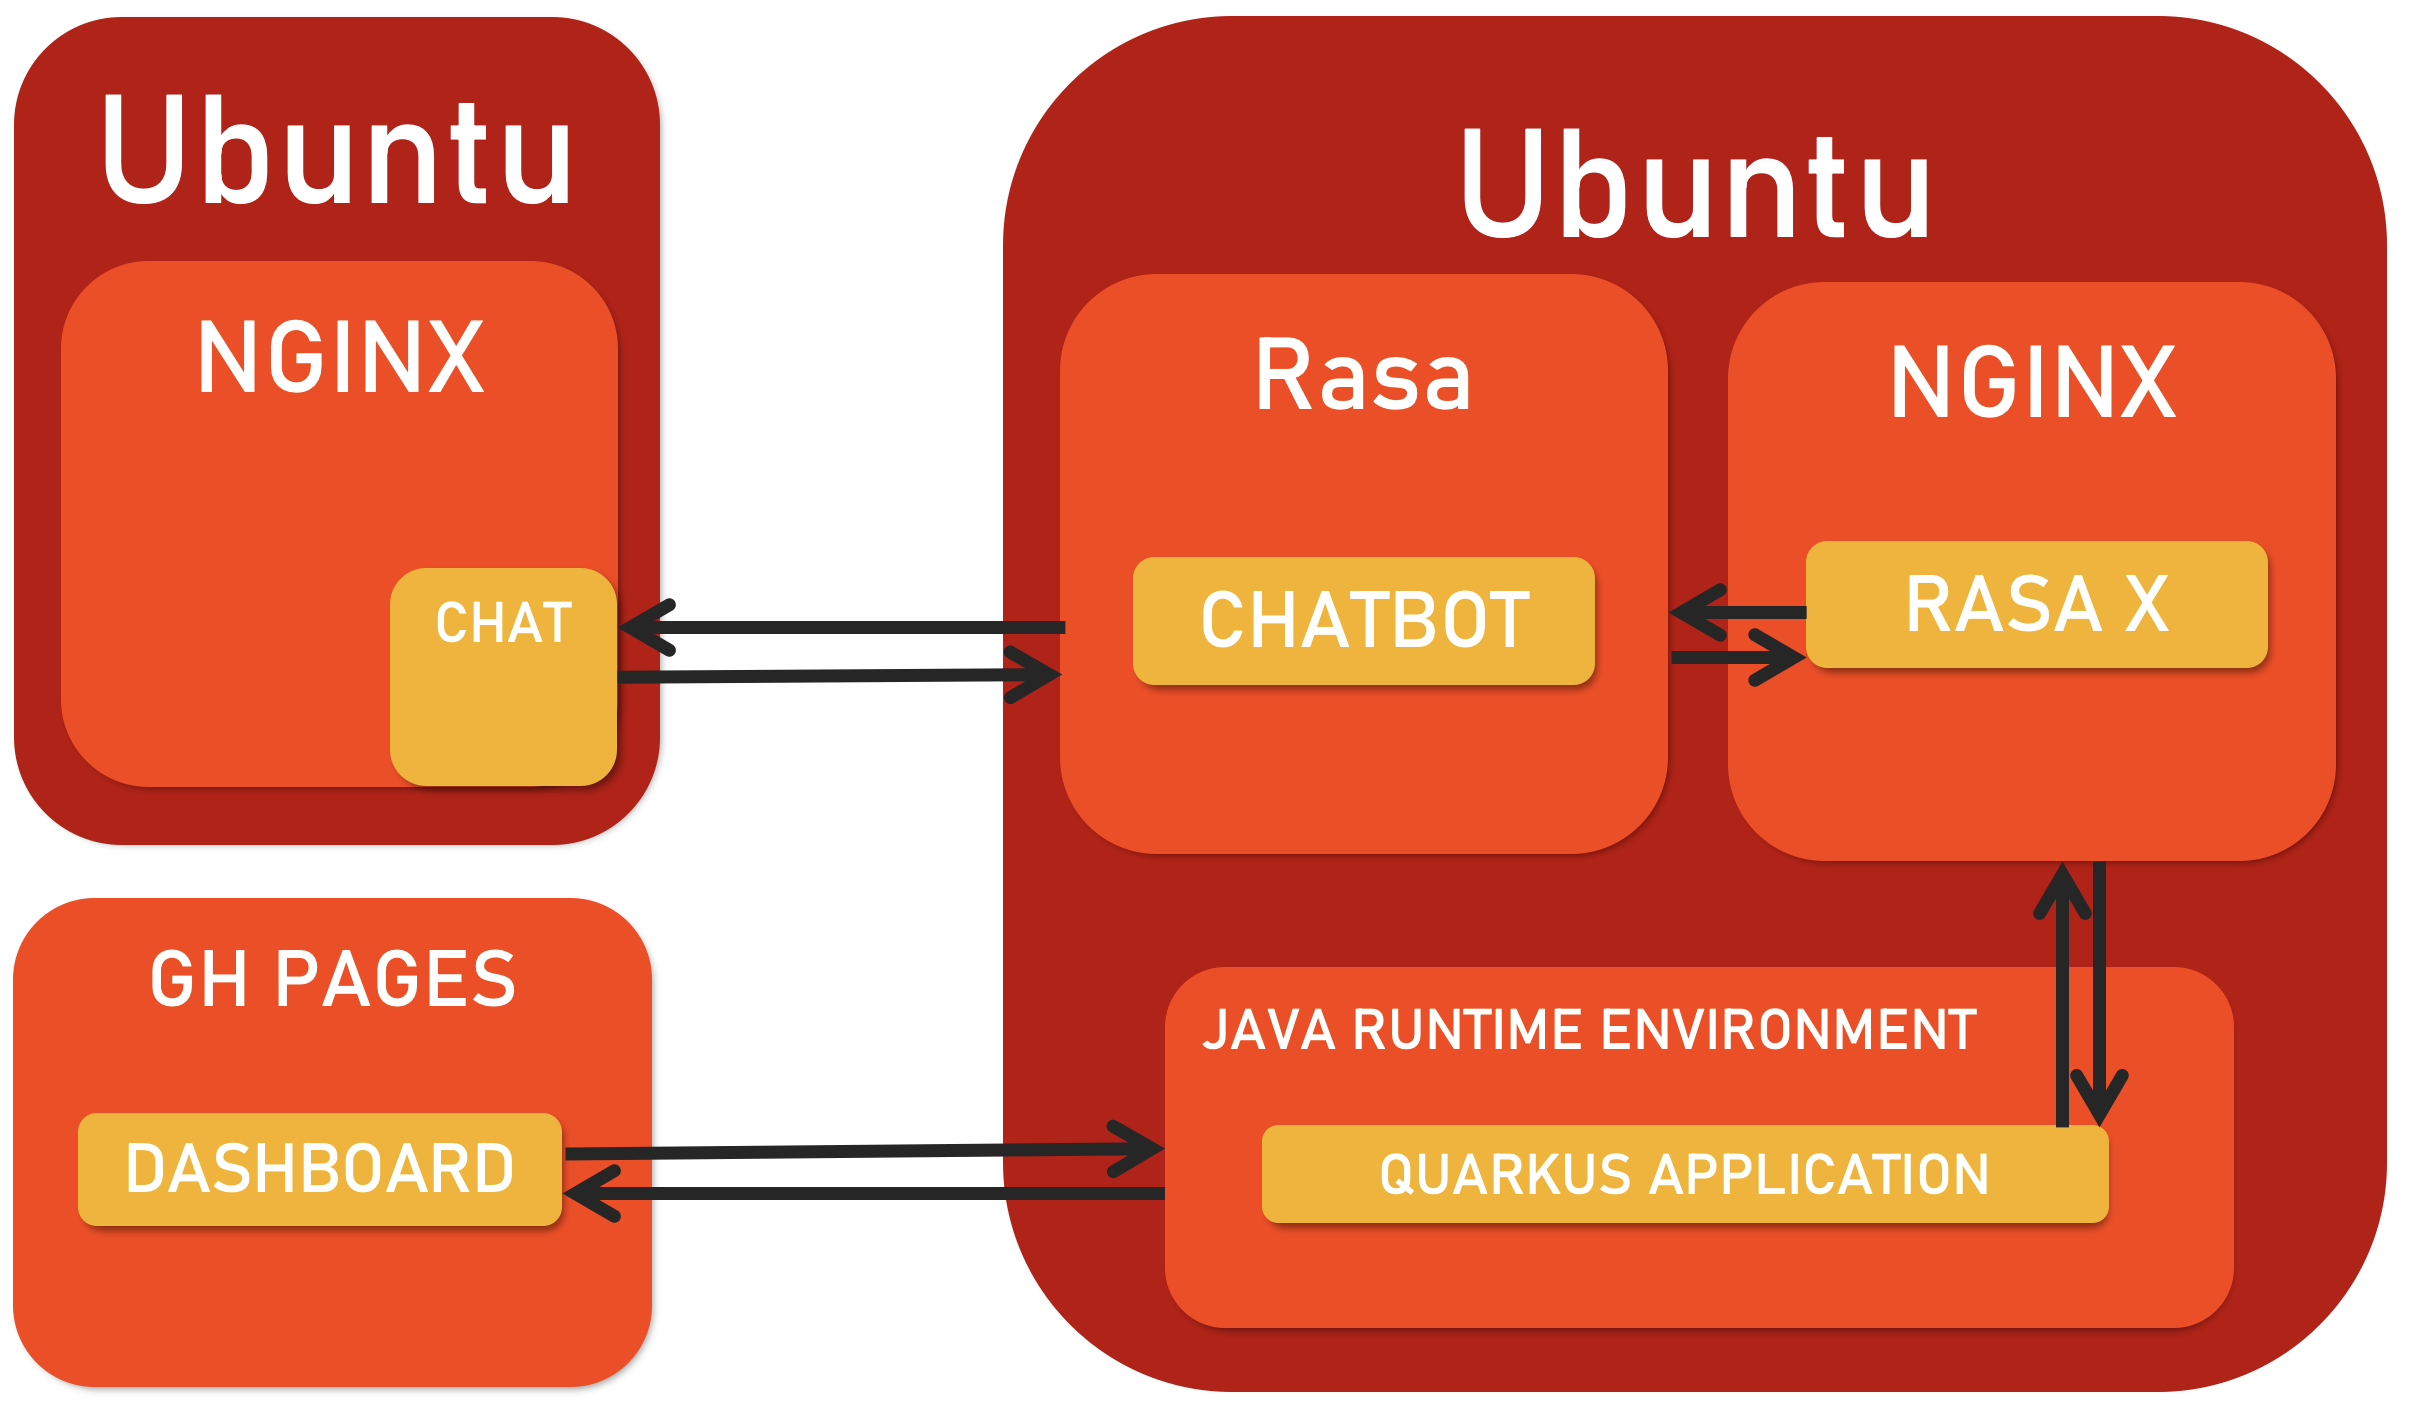
\includegraphics[scale=0.2]{pics/systemarchitektur}
    \caption{Systemarchitektur}
    \label{fig:impl:architektur}
\end{figure}

Wir haben 2 Ubuntu VM's, eine für den Chat und eine für Rasa und das Backend, nachdem der Chat auf die HTL Leonding Seite kommt, wird dadurch nur noch eine VM benötigt.

Unser Chat wird gerade mit NGINX gehostet, dieser kommuniziert mit Rasa direkt über REST, wenn der Benutzer eine Nachricht sendet, wird diese an Rasa gesendet und Rasa antwortet mit der passenden Antwort.
Das Dashboard wird auf GH Pages gehostet, dieses kommuniziert mit dem Backend über REST, das Backend authentisiert sich bei Rasa X und holt sich alle Konversationen und bereitet diese auf und sendet sie an das Dashboard.

\section{Backend}\label{sec:backend}
\setauthor{Felix Dumfarth}

Unser Quarkus ~\ref{quarkus} Backend hat die Aufgabe mit Rasa X zu kommunizieren und die Konversationsdaten für das Dashboard aufzubereiten und zu senden.

Unser Backend besitzt folgende Endpoints:

\begin{itemize}
    \item GET /api/conversations
    \item GET /api/conversations/{id}
    \item POST /api/feedback
    \item GET /api/feedback
    \item GET /api/file/{filename}
    \item PUT /api/file/{filename}
\end{itemize}

Bei den beiden ``conversations'' endpoints muss man sich aber zuerst authentisieren und sich einen Bearer Token von Rasa x holen damit man auf die anderen Rasa X endpoints zugreifen kann .

\subsection{GET /api/conversations}
Der Endpoint ruft zuerst die getAuth() funktion auf, um den Bearer Token zu erhalten.

Danach wird der Rasa X GET Endpoint /api/conversations aufgerufen mit dem Bearer Token im Header.
Von diesem Endpoint wird ein JSON Objekt zurückgegeben, das die Konversationen enthält, aber zusätzlich noch viele andere unrelevante Daten, deshalb holt sich das Backend wirklich nur ID des Senders, die Zeit und die Anzahl von Nachrichten der Unterhaltungen.

\subsection{GET /api/conversations/{id}}
Der Endpoint /api/conversations/{id} ruft zuerst die getAuth() funktion auf, um den Bearer Token zu erhalten.

Um nur von einer gezielten Unterhaltung die Nachrichten zu erhalten wird der Rasa X Endpint /api/conversations/{id}/messages aufgerufen mit dem Bearer Token im Header.
Die Response wird auch in dieser Form schon zurückgeben, da die Response keine unwichtigen Daten enthält.

\subsection{POST /api/feedback}
Der Endpoint /api/feedback erhält ein JSON Objekt mit den Daten des Feedback Formulars und speichert diese in die Datenbank.

\subsection{GET /api/feedback}
Der Endpoint /api/feedback liest alle Feedbacks aus der Datenbank und gibt diese zurück.

\subsection{GET /api/file/{filename}}
Der Endpoint /api/file/{filename} liest die im URL angegeben Datei aus dem Filesystem aus und gibt diese zurück.
Die möglichen Dateinamen sind:

\begin{itemize}
    \item nlu.yml
    \item rules.yml
    \item stories.yml
    \item config.yml
    \item domain.yml
\end{itemize}

\subsection{PUT /api/file/{filename}}
Der Endpoint /api/file/{filename} erhält den Inhalt aus dem File welches auch im URL angegeben wurde und überschreibt dieses dann im Filesystem.

\section{Chat Widget}\label{sec:chat-widget}
Der Chatbot der HTL Leonding sollte auf der Schulhomepage als Chatblase angezeigt werden, und verschiedene Elemente wie Buttons und Links unterstzützen.

\subsection{Konzept}
Während den Anfängen der vorliegenden Arbeit wurde ein Konzept erstellt, um das mögliche Aussehen festzulegen. Lange Zeit wurde der Chatbot unter den Namen Leon geführt.
Dies wurde jedoch im späteren verlauf geändert und Leon wurde Teil des langjährigen Leonie Projektes der HTL Leonding.
Ursprünglich war das Symbol des Chatbots, wie man am Konzept sehen kann, ein Bot. Durch den wechsel in die Leonie Familie wurde dieses Logo jedoch gegen Leonie getauscht.
\begin{figure}[hbt!]
    \centering
    \includegraphics[scale=0.2]{pics/conceptBotClosed.png}
    \caption{Konzept Chatbot geschlossen}
    \label{fig:impl:conceptBotClosed}
\end{figure}
\begin{figure}[hbt!]
    \centering
    \includegraphics[scale=0.2]{pics/conceptBotOpen.png}
    \caption{Konzept Chatbot geöffnet}
    \label{fig:impl:conceptBotOpen}
\end{figure}

\subsection{Umsetzung}
Umgesetzt wurde das Frontend mithilfe von Angular. Die Chatblase ist eine eigene Komponente, die durch CSS immer rechts unten fixiert ist. Die Farben des Chatbots sollten natürlich an die HTL Leonding erinnern, deshalb wurde ein Farbverlauf aus Farben des HTL Logos erstellt.

Jedoch begann der Chatbot sehr anders, zu begin wurde der Bot zuerst als ganze Seite entwickelt und nicht nur als Chatblase.
\begin{figure}[hbt!]
    \centering
    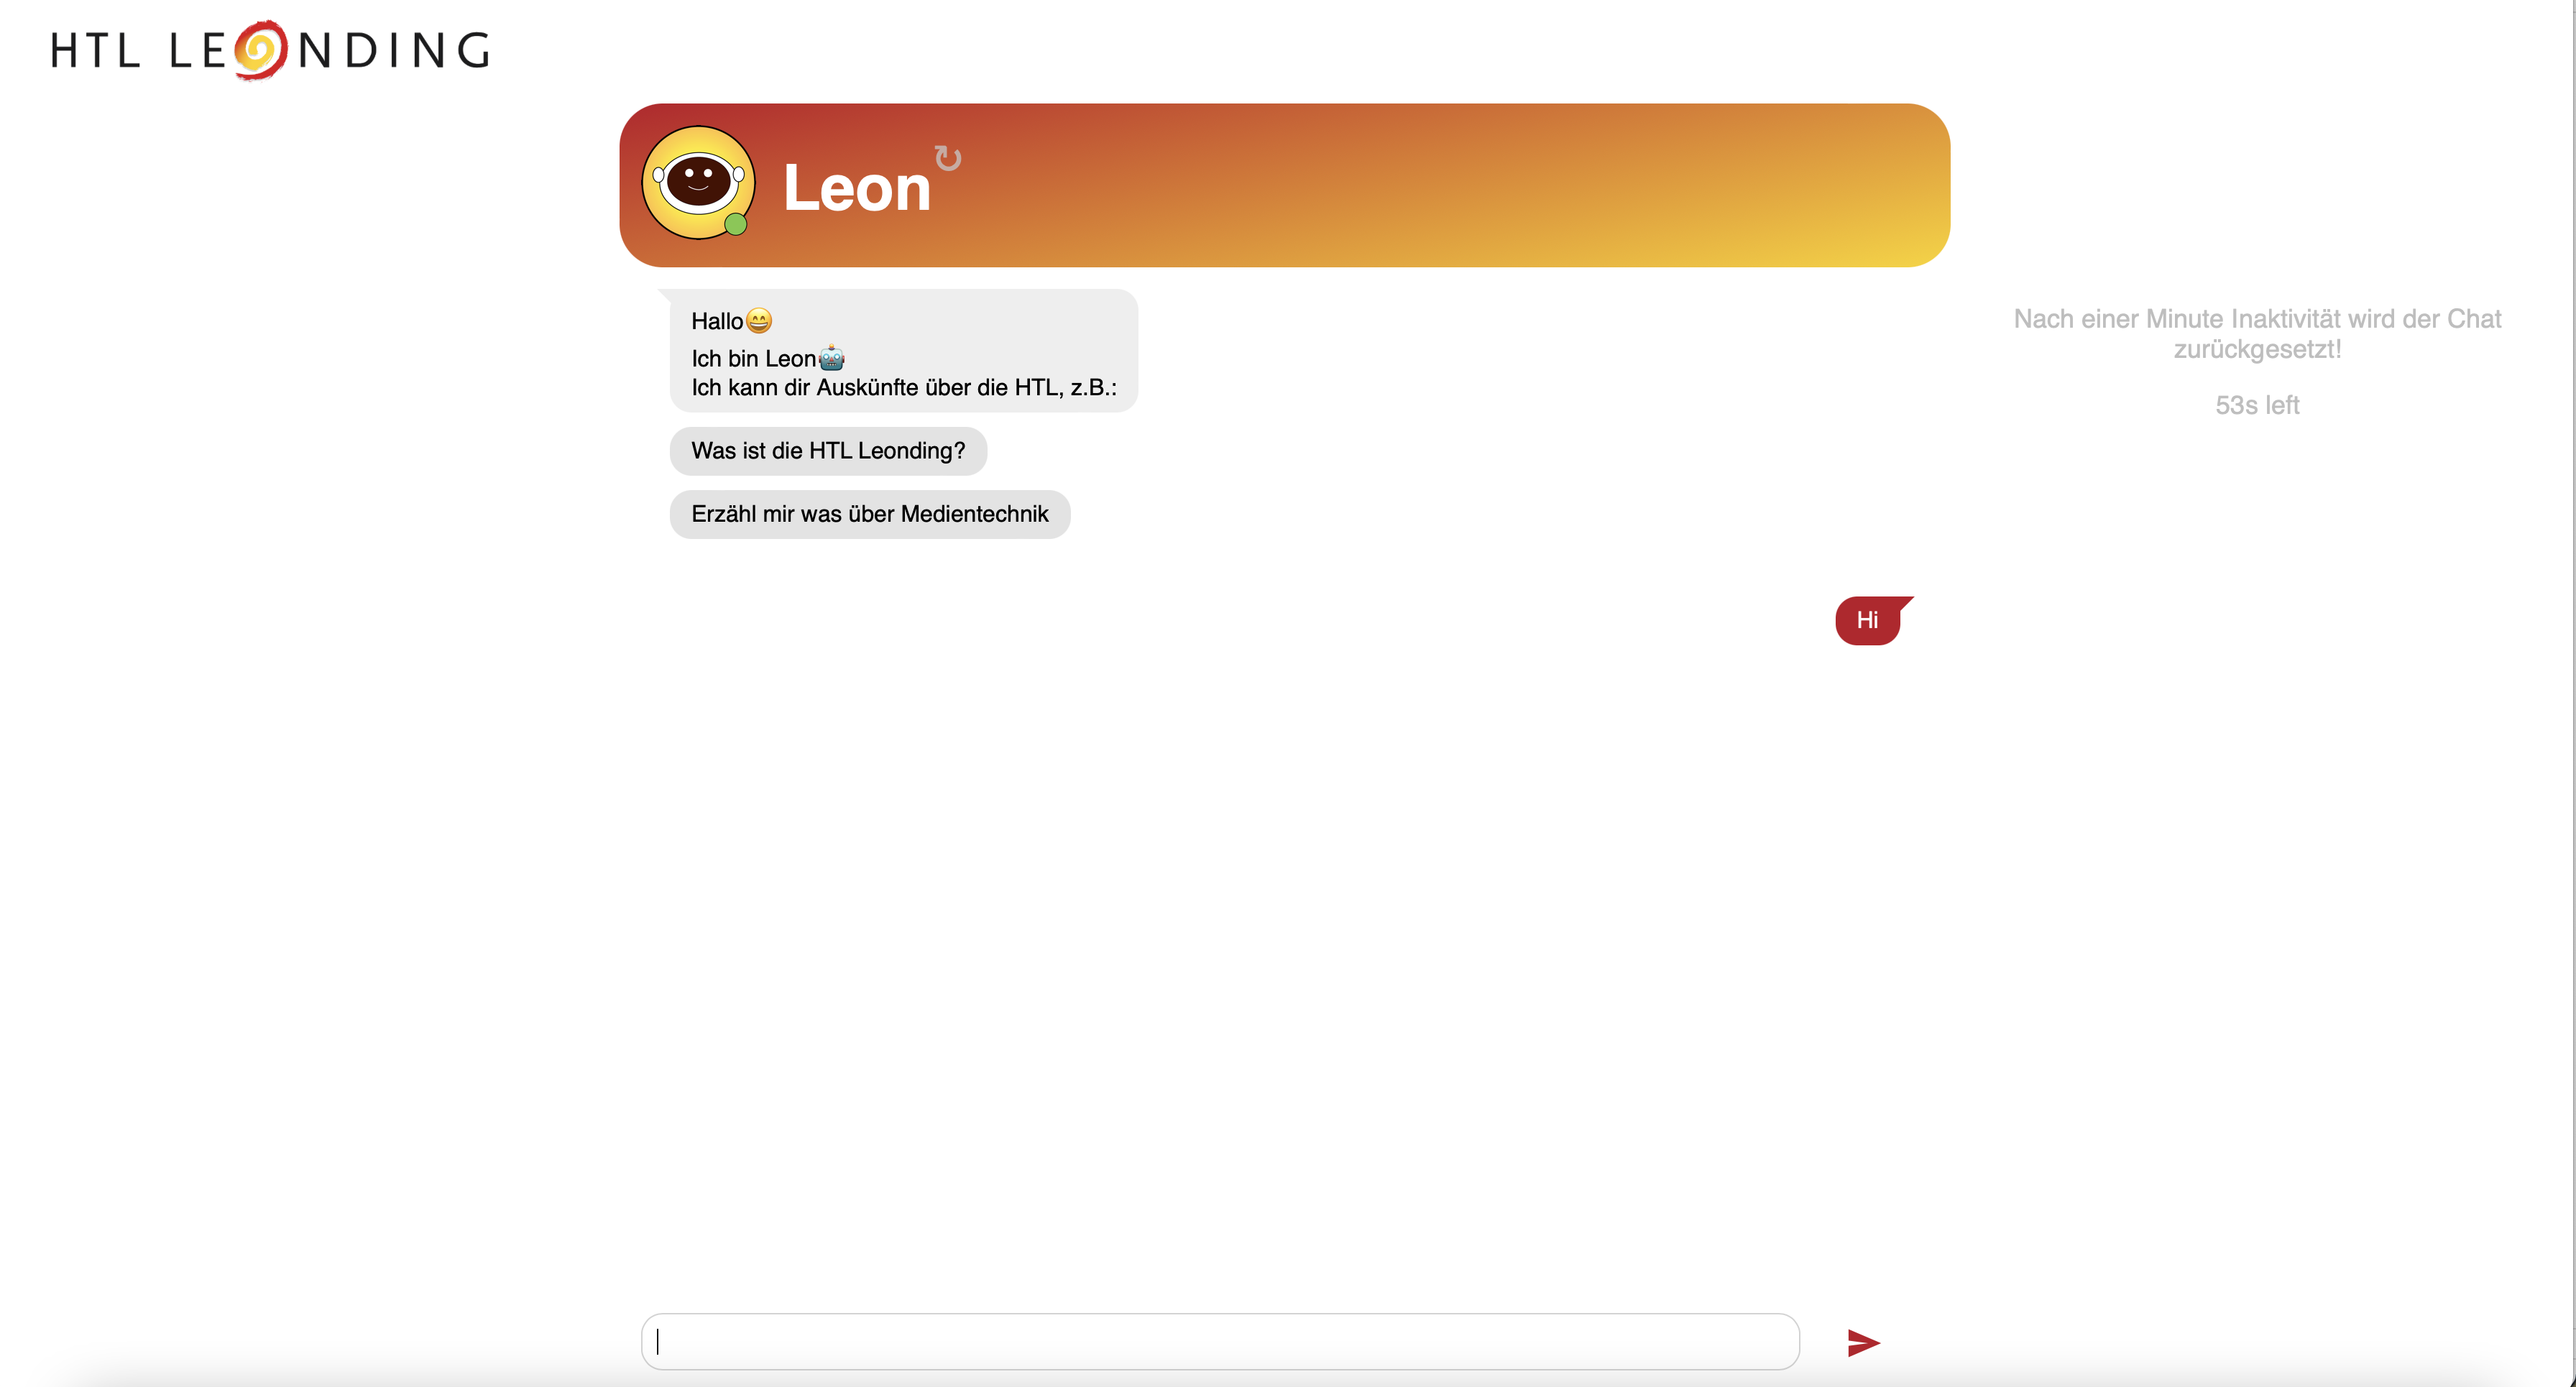
\includegraphics[scale=0.2]{pics/fullPageBot.png}
    \caption{Chatbot auf einer ganzen Seite}
    \label{fig:impl:conceptBotFullPage}
\end{figure}

Natürlich war dies nicht das endgültige Ziel so wurde der Bot schnell zur Chatblase umgewandelt.
Zum Testen war die HTL Leonding Seite mithilfe eines IFrames eingebunden und zusätzlich die Chatblasen Komponente.

Um das Gespräch in eine Richtung zu lenken wurden Buttons eingeführt, die nach fast jeder Antwort mögliche folge Fragen vorschlagen.

\begin{figure}[hbt!]
    \centering
    \includegraphics[scale=0.2]{pics/finalBot.png}
    \caption{Chatbot}
    \label{fig:impl:bot}
\end{figure}

Um Bewertungen von echten Benutzern zu holen wurde außerdem eine Feedback Seite eingeführt, in dieser kann der Benutzer eine 1 bis 5 Sterne bewertung und einen Text absenden.

%TODO: Bilder zum Feedback


Die Chatblase wurde in einem eigenen Modul entwickelt, um die Komponenten zu verstecken und zu verbergen.

Das Chatfenster wurde in 3 Bereiche geteilt.

\begin{figure}[hbt!]
    \centering
    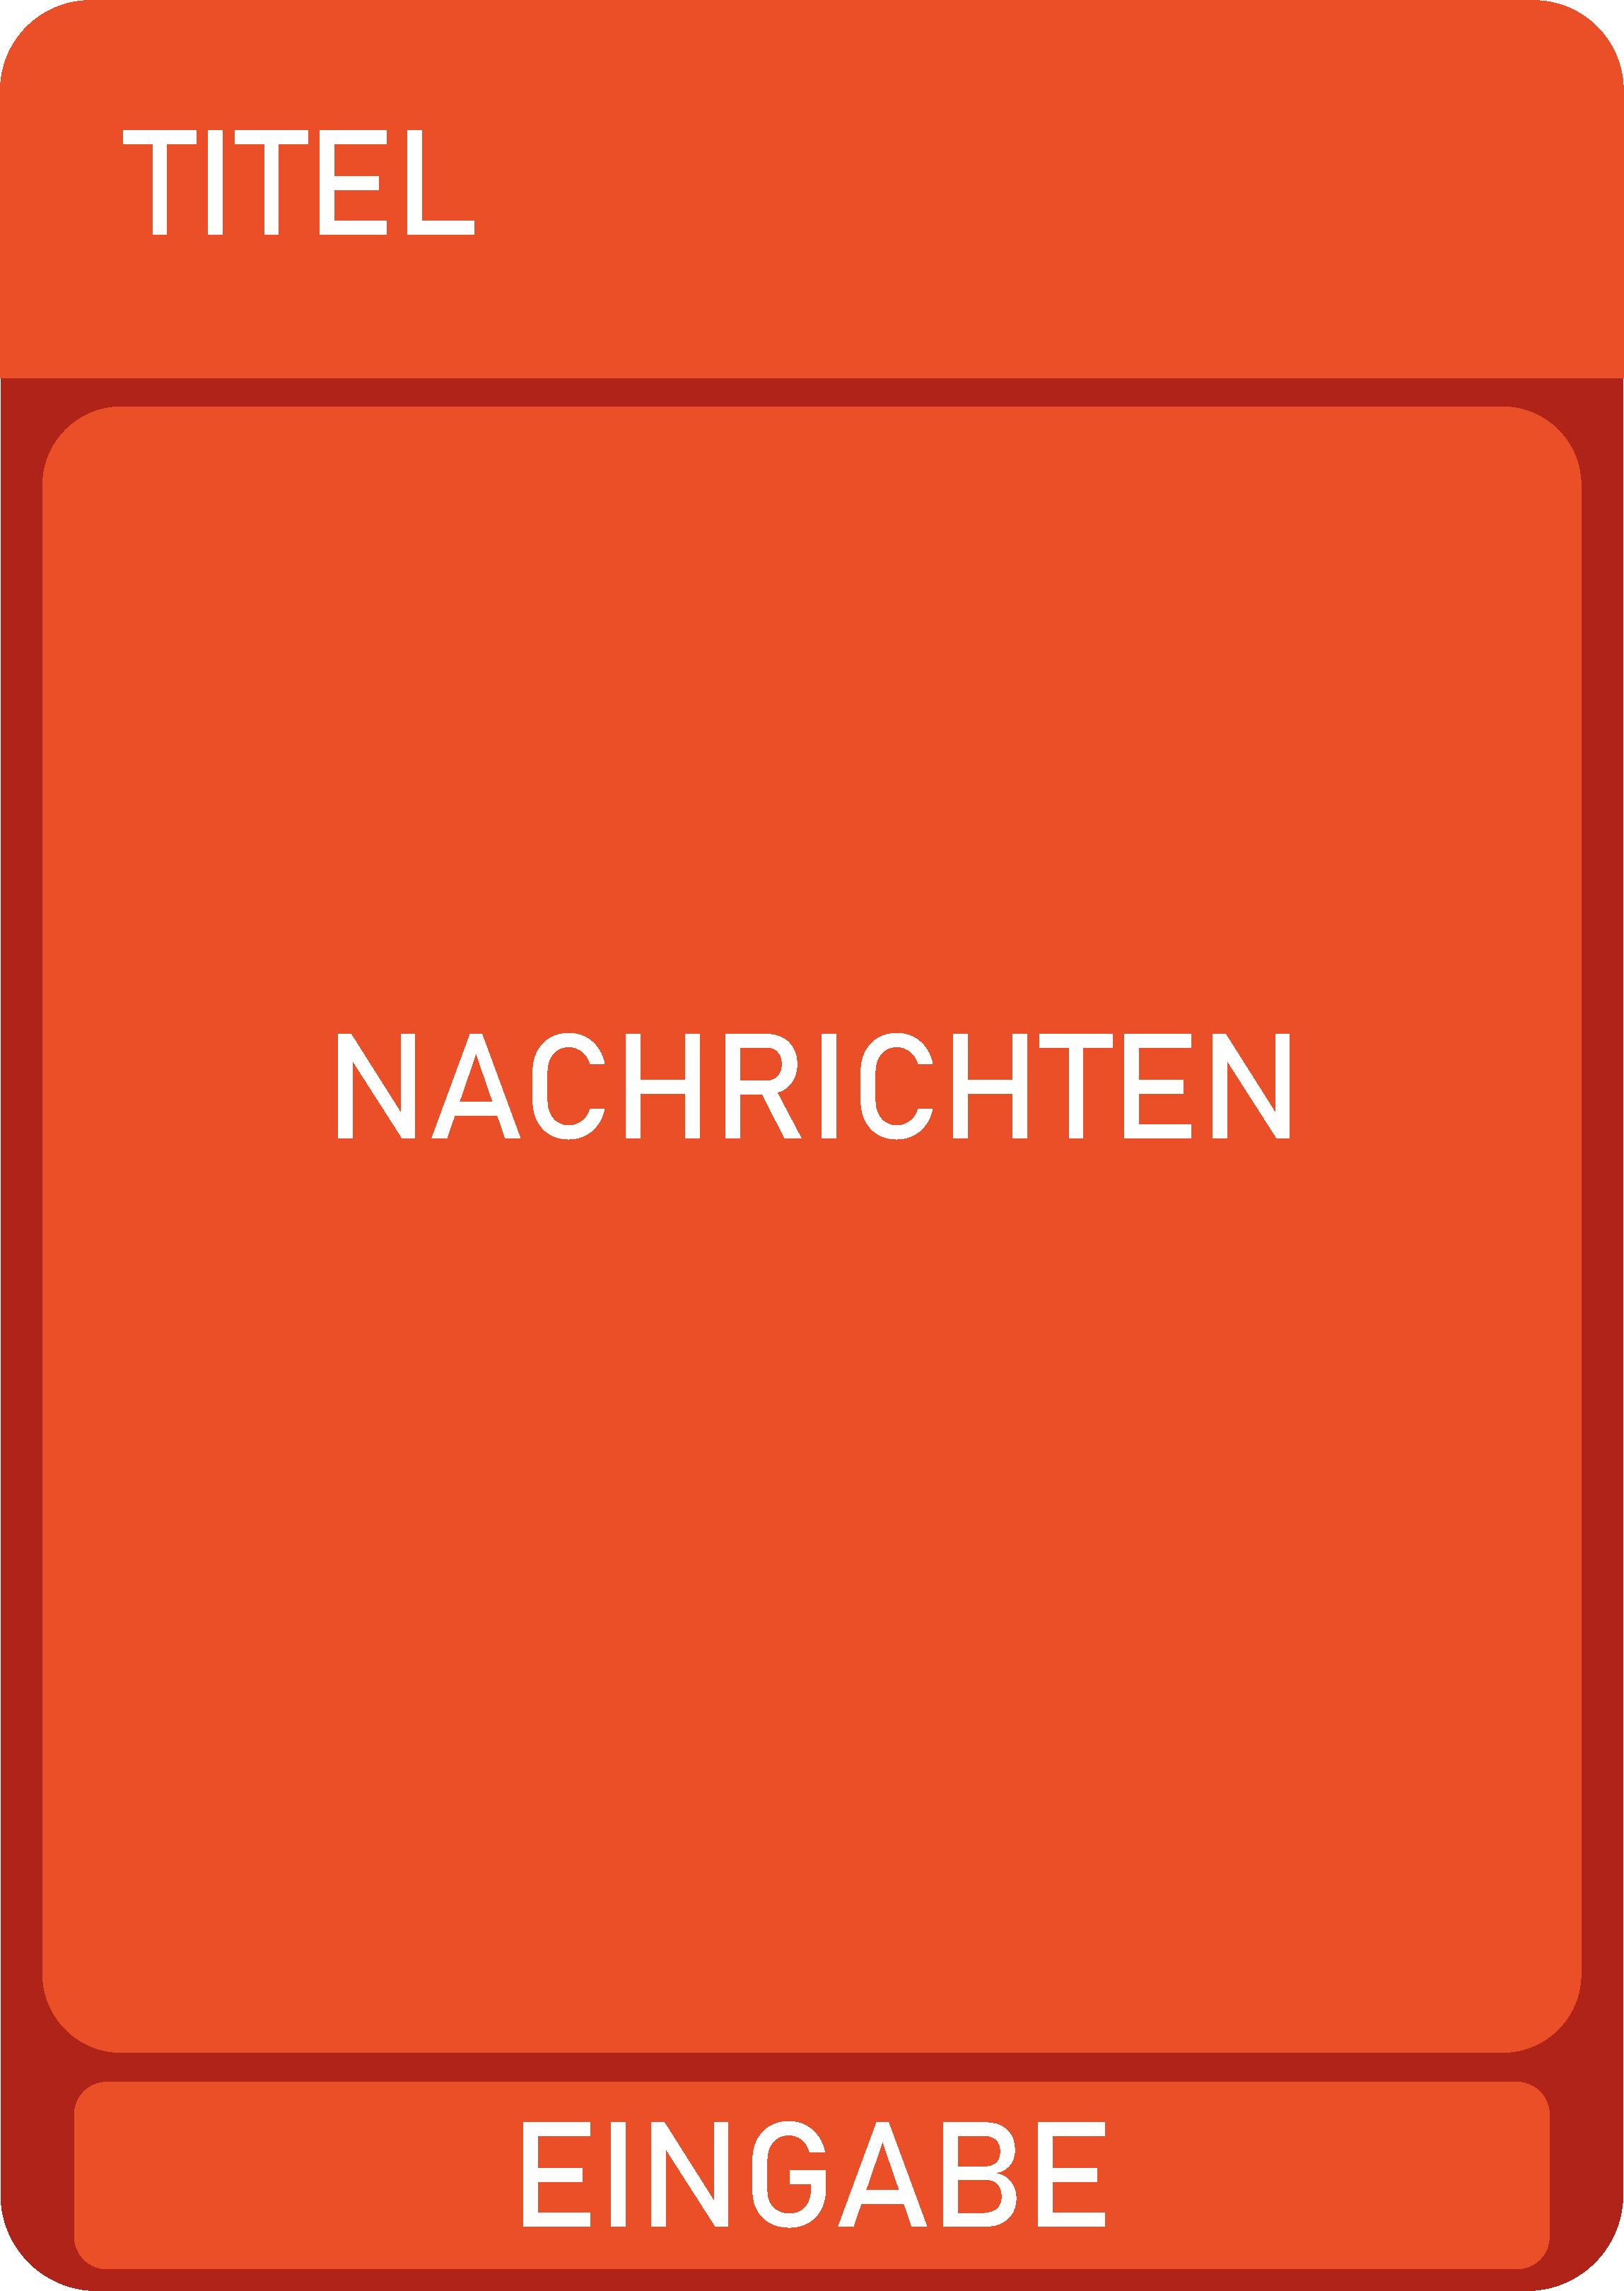
\includegraphics[scale=0.2]{pics/chatWidgetStructure}
    \caption{Aufbau vom Chat Fenster}
    \label{fig:impl:chatWidget}
\end{figure}


\section{Dashboard}\label{sec:dashboard}

Um alle Gespräche und die Bewertungen der Benutzer anzuzeigen wurde ein Dashboard eingeführt, wo nur dies möglich war.
Im Laufe der Arbeit wurde dieses dann erweitert, um für den Leobot Conversation Cycle als Seite zu dienen.

\subsection{Conversation-Driven Development}\label{cdd}
Rasa empfiehlt für die Entwicklung von Chatbots ``Conversation-Driven Development'', kurz CDD.\cite{cdd}
Aber was ist CDD?

CDD beschreibt eine Entwicklungsstrategie, in der du deinen Chatbot nach Konversationen mit echten Usern verbesserst.

Bei CDD wird empfohlen, dass man seinen Chatbot möglichst früh echten Benutzern zur verfügung stehlt und so beobachten kann was die echten Benutzer alles für Intents erwarten und wie sie ihre Anfragen formulieren und kann diese bei Bedarf hinzufügen.



\subsection{Leobot Conversation Cycle}

\begin{figure}[hbt!]
    \centering
    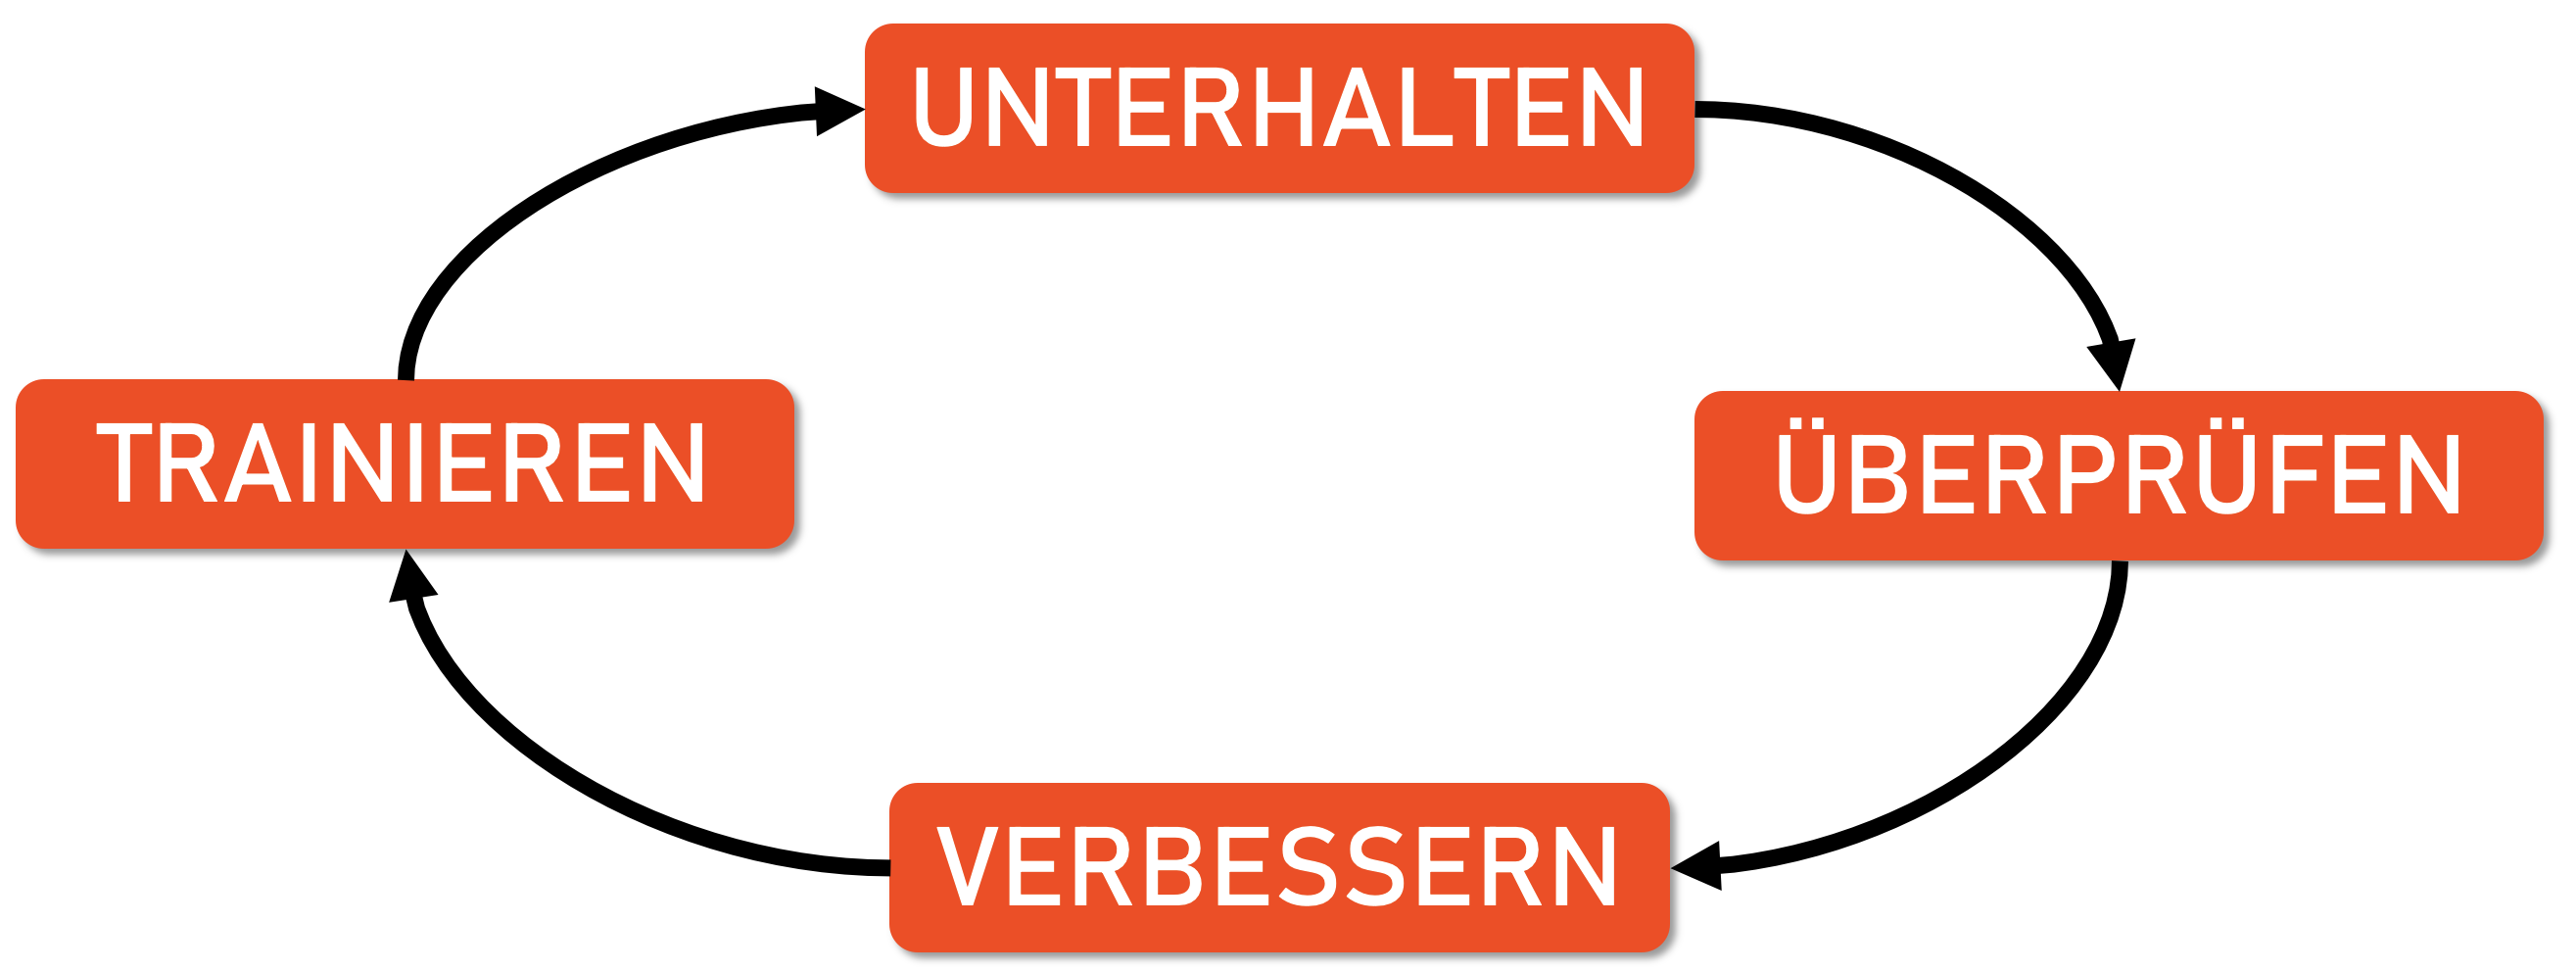
\includegraphics[scale=0.2]{pics/LeoCircle}
    \caption{Leobot Conversation Cycle}
    \label{fig:impl:ConversationCycle}
\end{figure}

Wir setzen CDD ~\ref{cdd} mithilfe unsres Leobot Conversation Cycle um, der Leobot Conversation Cycle ist ein Workflow, der dazu dient, den Leobot zu überprüfen und zu erweitern.

Der Workflow besteht aus folgenden Schritten:

\begin{itemize}
    \item Unterhalten
    \item Überprüfen
    \item Verbessern
    \item Trainieren
\end{itemize}

Diese 4 Schritte werden immer wieder durchgeführt um den Chatbot dauerhaft zu verbessern.

\subsubsection{Unterhalten}
Unterhalten ist der erste Schritt des Leobot Conversation Cycles, in diesem Schritt werden dem Bot Fragen gestellt, die er beantworten muss, dies passiert natürlich während Unterhaltungen im Chat auf der Schulhompage.
Die Unterhaltungen werden dann alle gespeichert.

\subsubsection{Überprüfen}
Überprüfen ist der zweite Schritt des Leobot Conversation Cycles, in diesem Schritt wird der Bot überprüft, ob er die Fragen richtig beantwortet und erkannt hat.
Dieser Schritt wird von Verantwortlichen für den Leobot durchgeführt.

\subsubsection{Verbessern}
Verbessern ist der dritte Schritt des Leobot Conversation Cycles, in diesem Schritt wird der Bot verbessert, das heißt die Fehler werden versucht zu beheben.
Je nachdem was der fehler des Bots war muss hier anders gearbeitet werden.
Wenn er einen Intent den er eigentlich kennt aber die Formulierung des Benutzers so war das er diesen nicht erkannt hat, wird die Eingabe des Benutzers zu den Trainingsdaten hinzugefügt.

Falls jemand aber eine Frage stellt zu der es keinen Intent gibt und sich die Verantwortlichen denken es wäre ein guter Intent so wird der ganze Intent zu den Trainingsdaten hinzugefügt.

\subsubsection{Trainieren}
Trainieren ist der vierte Schritt des Leobot Conversation Cycles, in diesem Schritt werden die Trainingsdaten an den Bot übergeben und dieser Trainiert und wechselt auf das neu trainierte Model.

Und nun beginnt der Leobot Conversation Cycle wieder von vorne.

\subsection{Umsetzung}

Einerseits kann man sich die vergangenen Unterhaltungen ansehen, so wie die nlu.yml, stories.yml, rules.yml, domain.yml direkt im Monaco Editor bearbeiten und speichern.

\begin{figure}[hbt!]
    \centering
    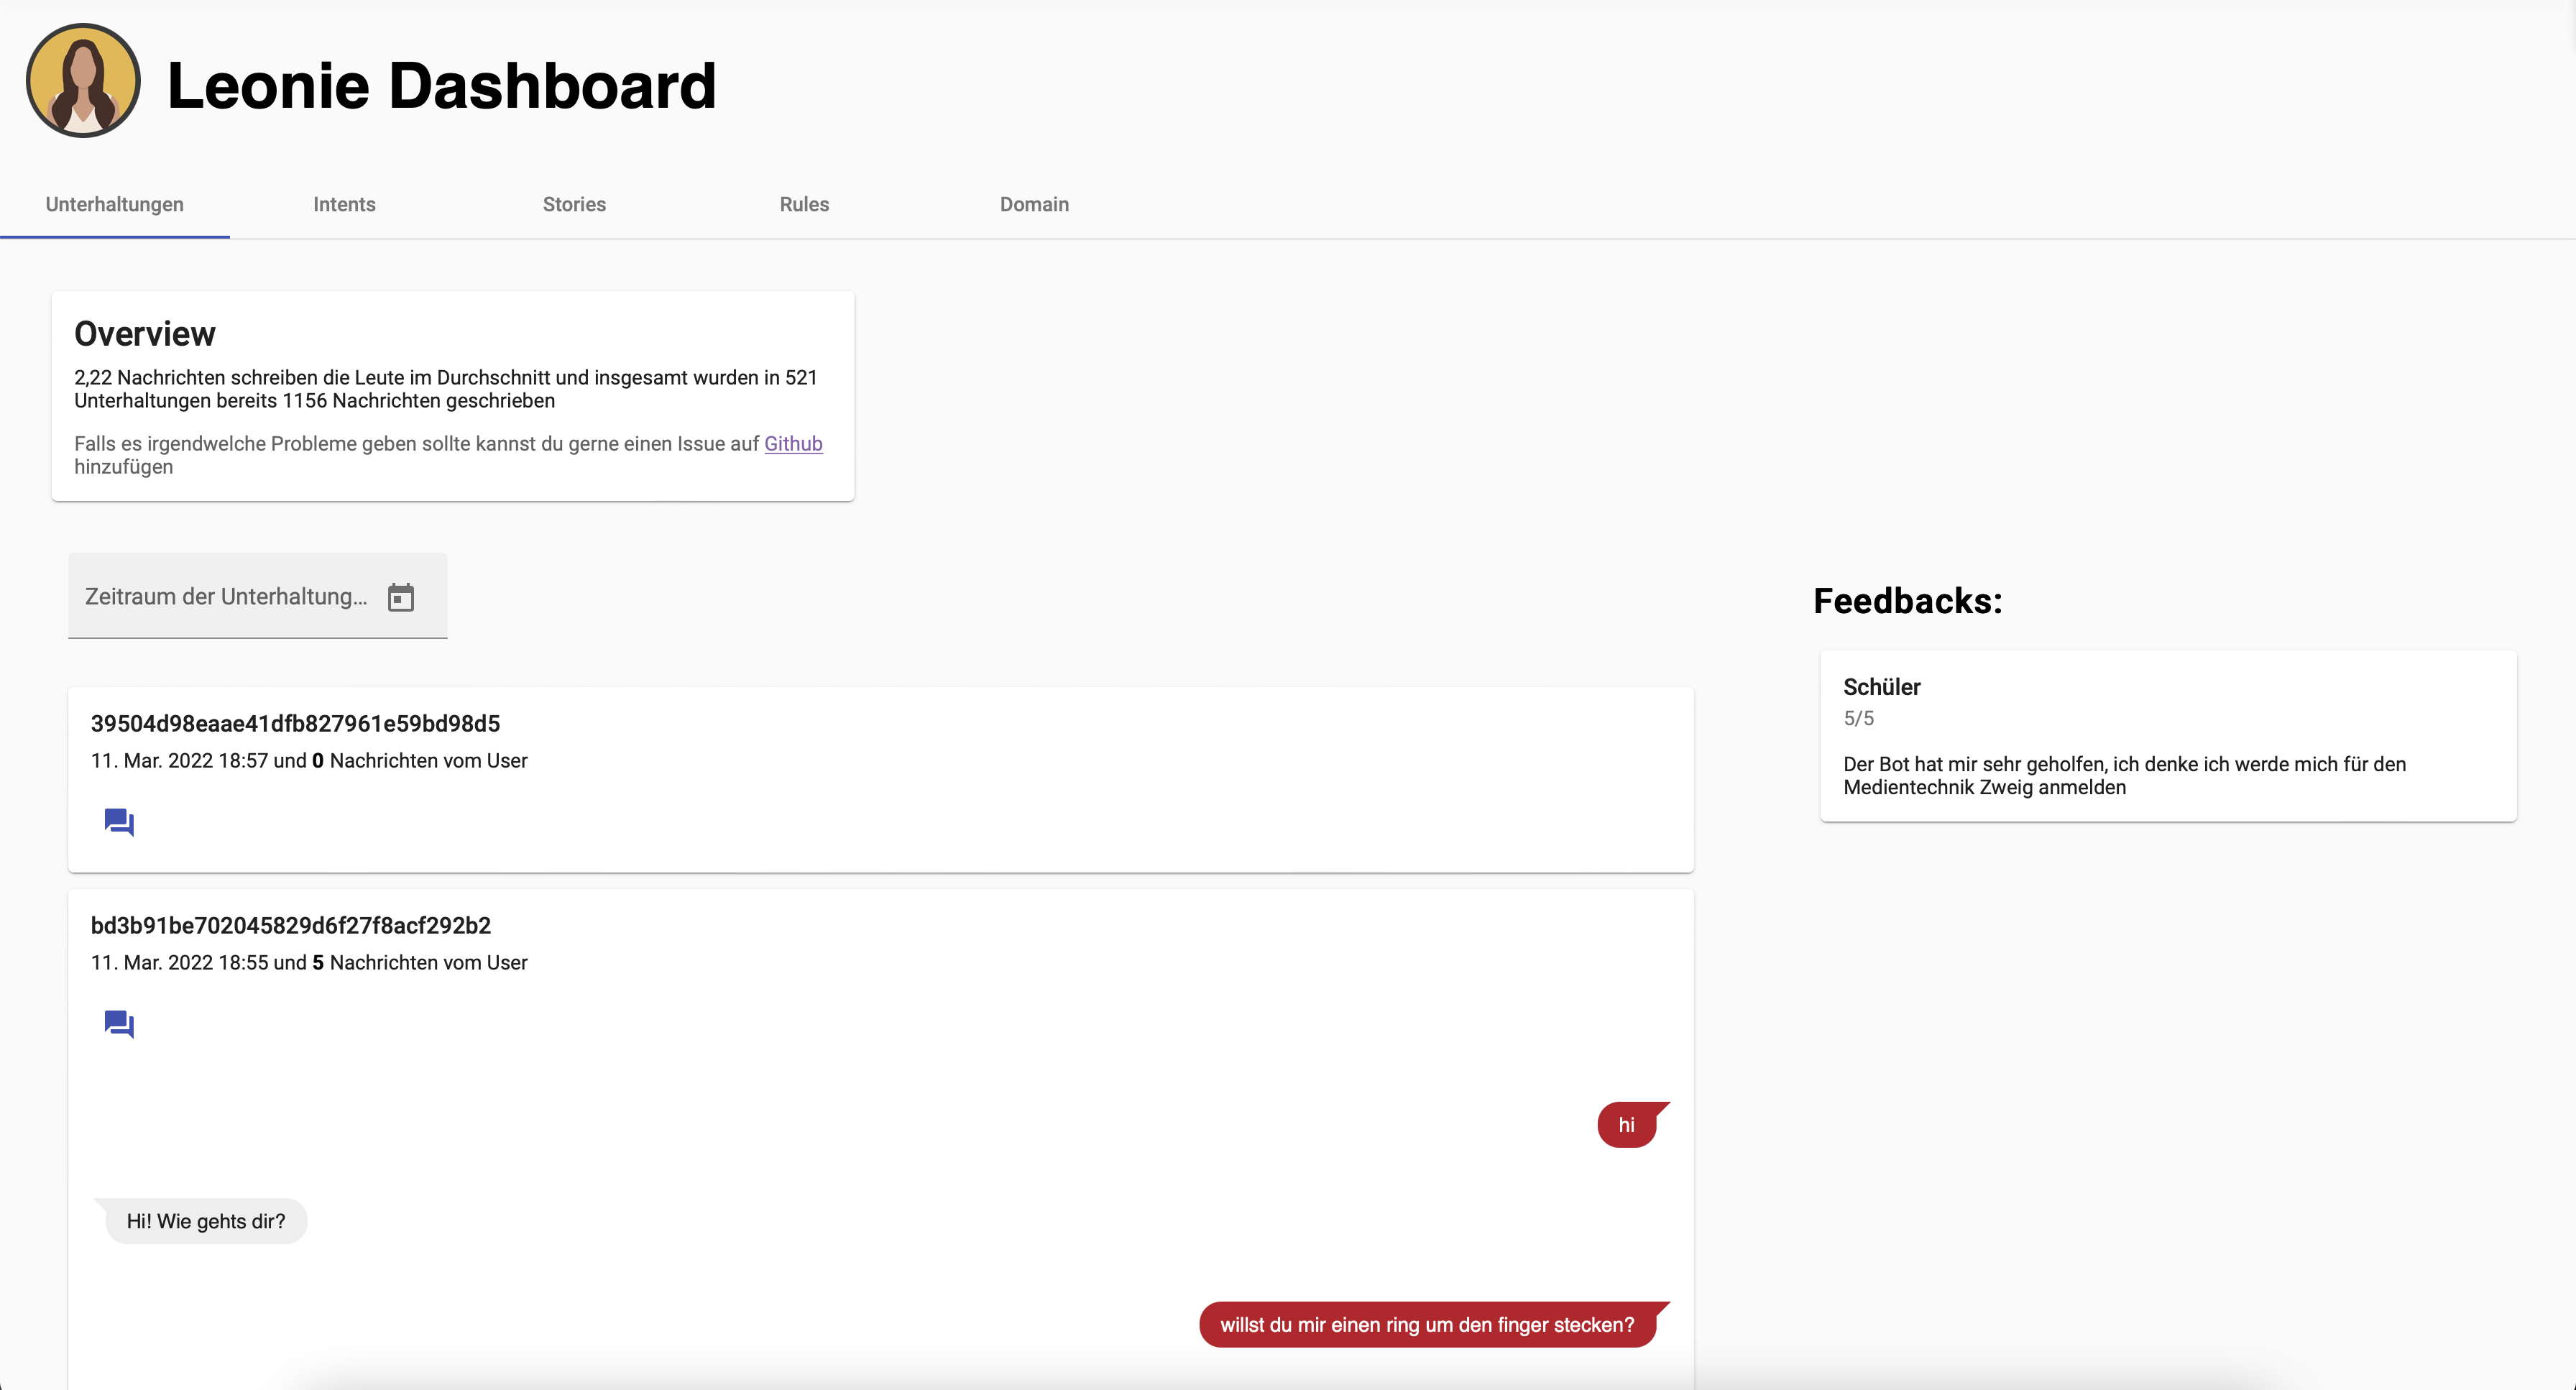
\includegraphics[scale=0.2]{pics/dashboardConvo}
    \caption{Dashboard}
    \label{fig:impl:dashConv}
\end{figure}

Im Editor wurden auch Code Vorschläge benutzt um etwas an Tipparbeit sparen zu können.

\begin{figure}[hbt!]
    \centering
    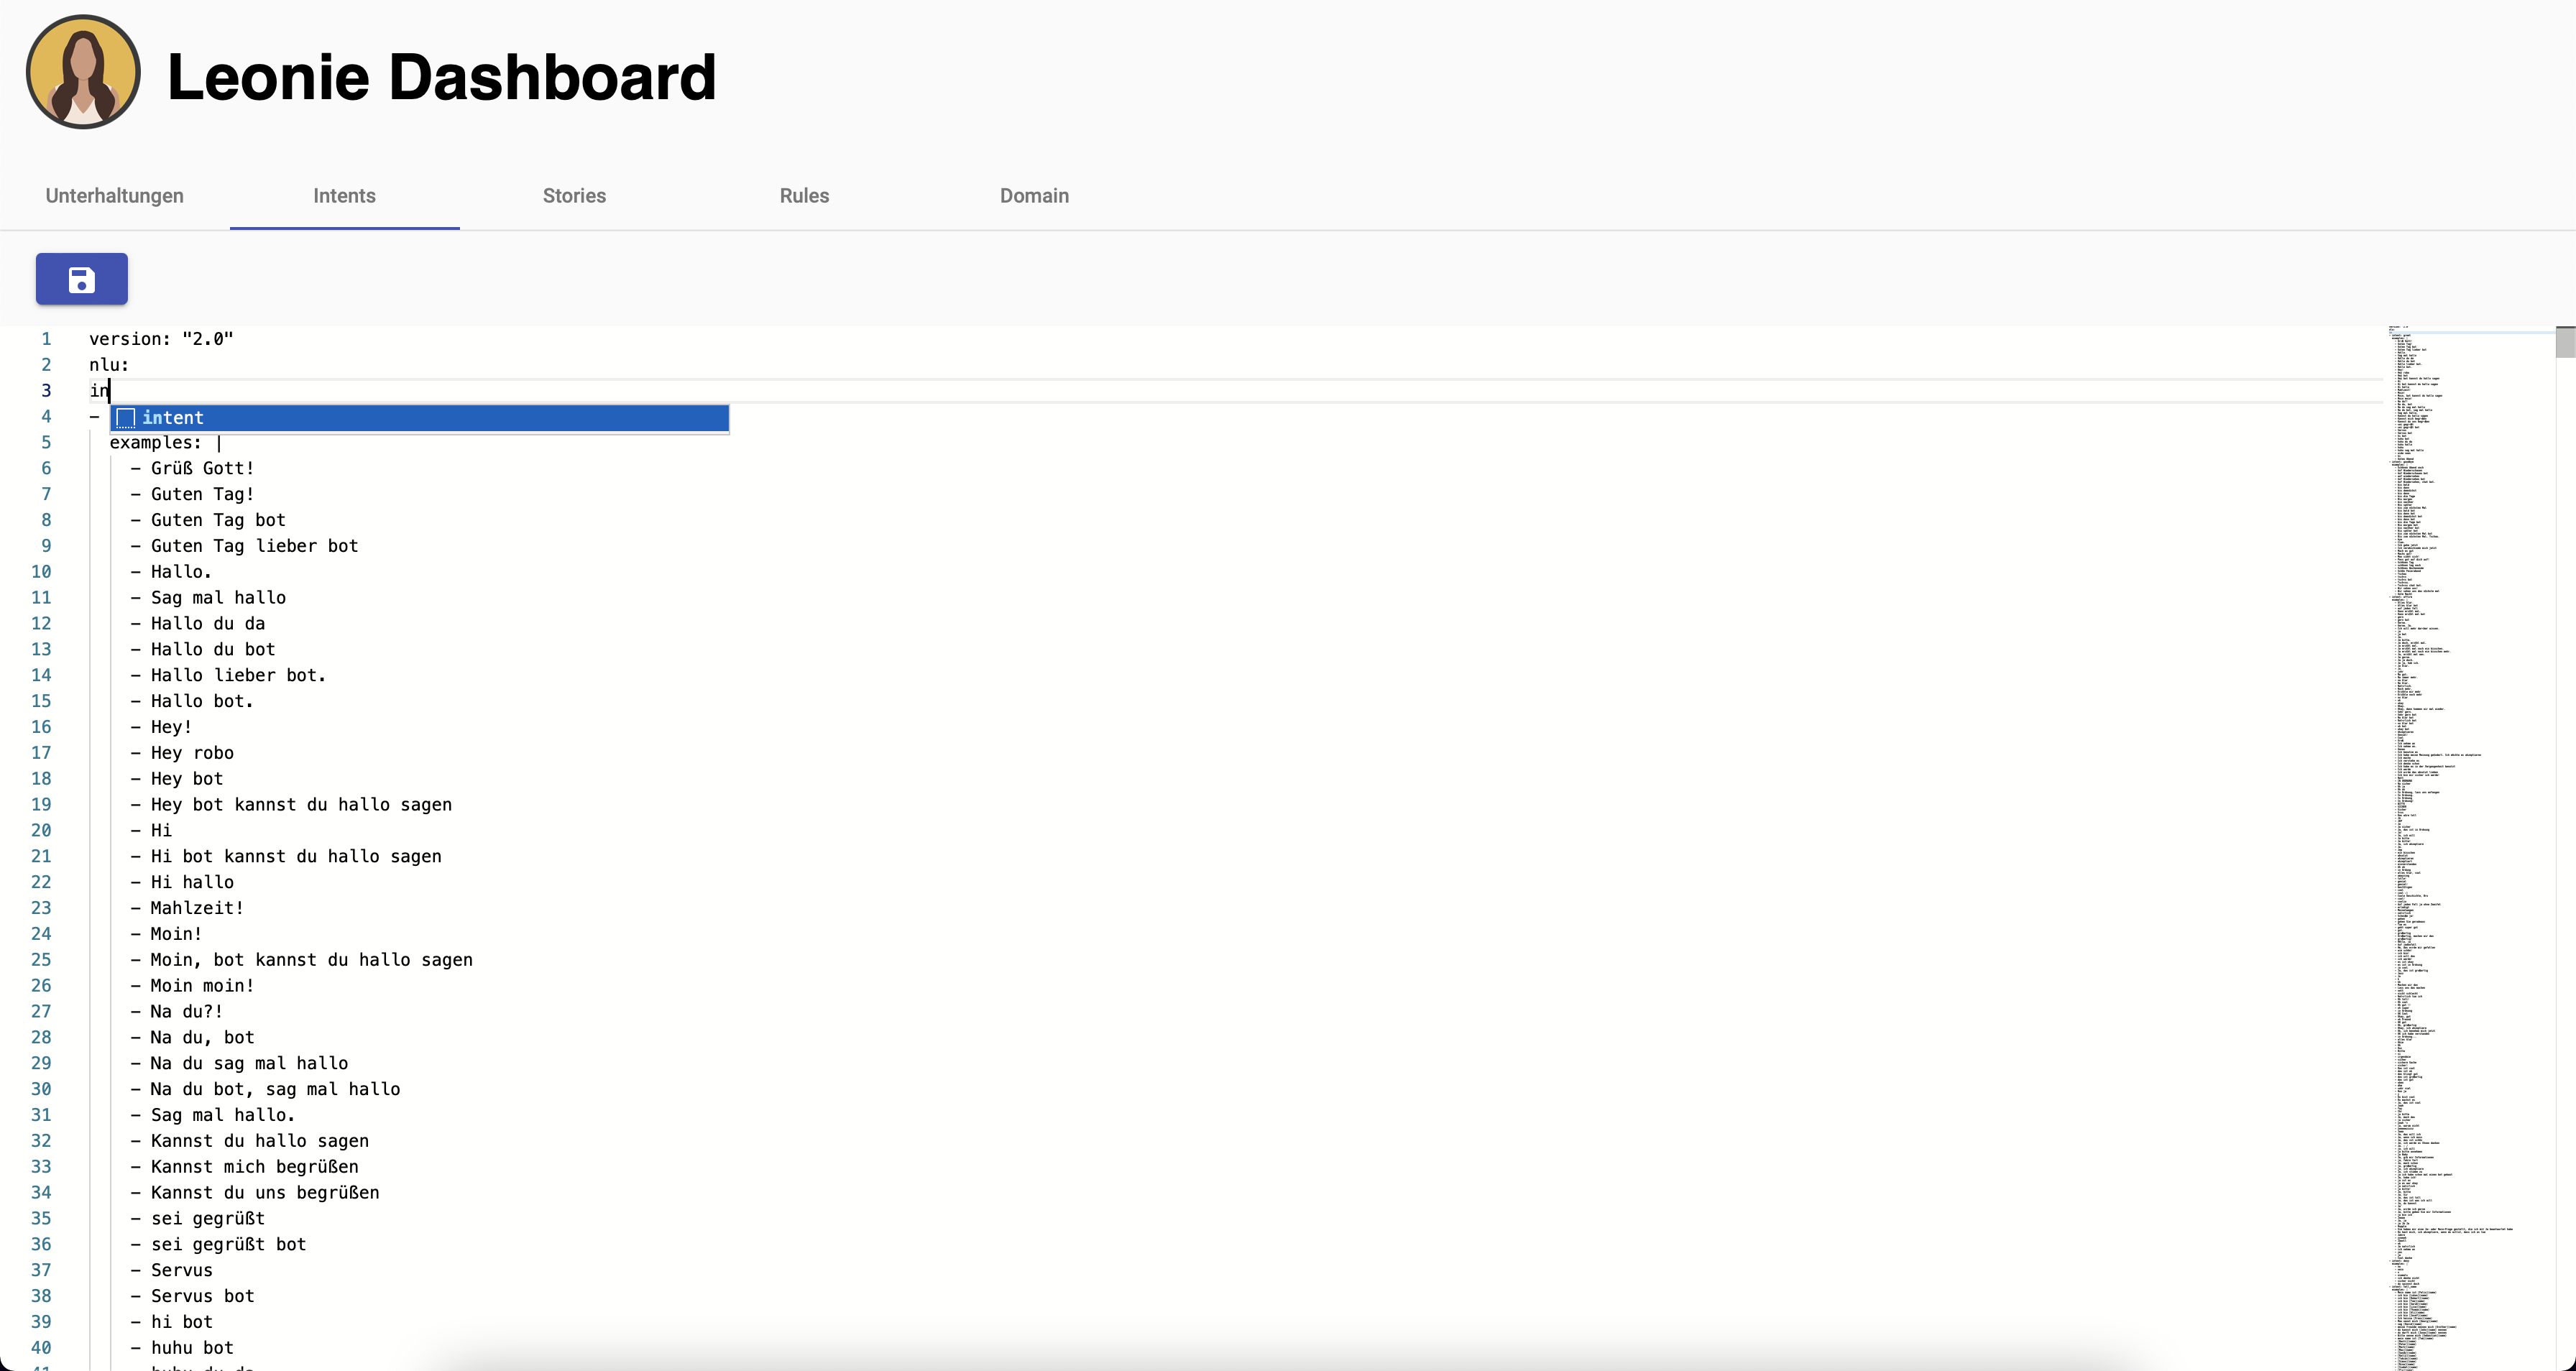
\includegraphics[scale=0.2]{pics/dashboardCodeSuggestion}
    \caption{Vorschläge}
    \label{fig:impl:dashboardCodeSuggestion}
\end{figure}
\begin{figure}[hbt!]
    \centering
    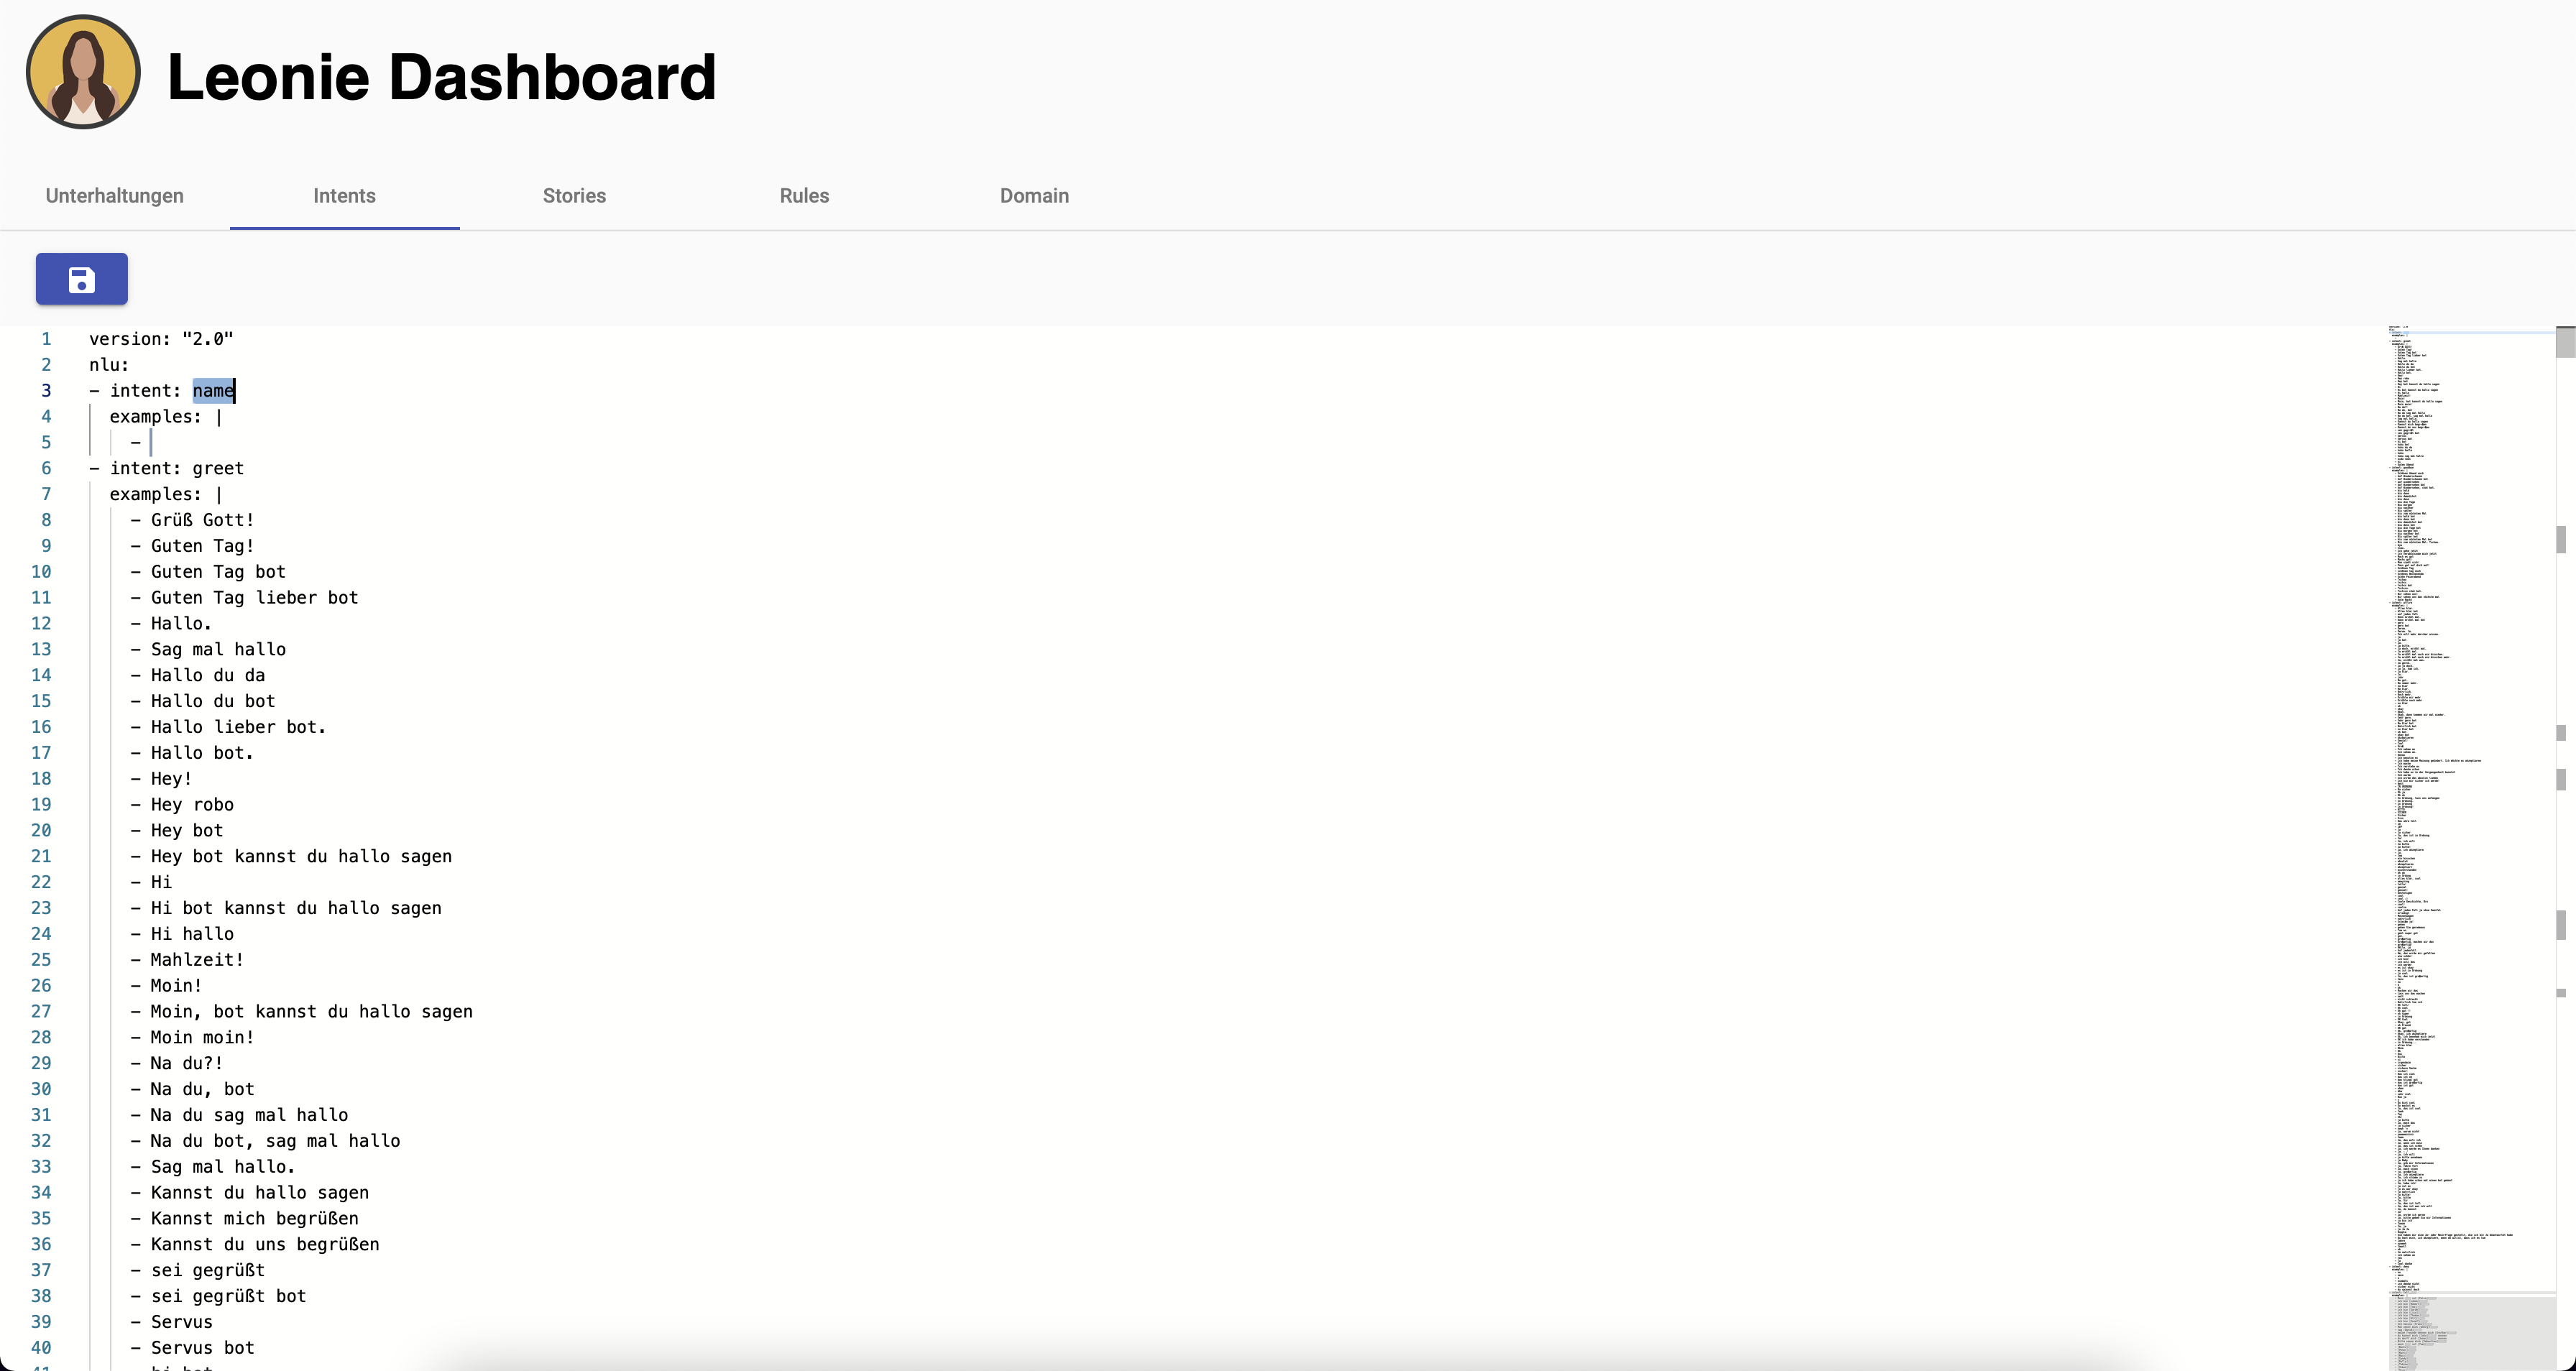
\includegraphics[scale=0.2]{pics/dashboardSuggestionMade}
    \caption{Vorschlag benutzt}
    \label{fig:impl:dashboardCodeSuggestionMade}
\end{figure}



\section{Einbindung in Wordpress}
\subsection{Angular Elements}
''Webkomponenten sind eine Gruppe von Web-Technologien, die es ermöglichen, benutzerdefinierte, wiederverwendbare HTML Elemente zu erstellen, deren Funktionalität gekapselt ist und damit vollständig getrennt von anderem Code.''\cite{webcomponents}

Um unsre Chatkomponente auf die Wordpress Seite zu bringen, entschieden wir uns dazu die Komponente mithilfe von Angular Elements als WebKomponente zu exportieren um somit eine einfache einbindung auf die Schulhomepage zu ermöglichen.

\section{GitHub Actions}

Die Praxische Arbeit besteht aus sehr vielen einzelen Projekten, mit verschiedenen Funktionen, doch bei vielen der GitHub Projekte haben wir mithilfe von GitHub Actions unser Deployment automatisiert.

% TODO
\subsection{Backend}

Unser Backend wird mithilfe von GitHub Actions automatisiert gebaut der Workflow baut das .jar file und dieses wird dann über SSH auf unsre VM geladen.

\subsection{Fronteend}
Die Chat Seite sowie das Dashboard werden mithilfe von GitHub Actions automatisiert gebaut und auf GH Pages gepublished.

\section{Schwierigkeiten}
\setauthor{Felix Dumfarth}

\subsection{Backend}
Beim Backend war eine sehr große Schwierigkeit, dass die Rasa X API nicht sehr gut dokumentiert ist und deshalb sehr vieles nur durch Probieren und sehr tiefe Recherchen ermittelt werden konnte.


\subsection{Frontend}
Beim Frontend war die größte Schwierigkeit der export der Chatkomponente da Angular Materials nicht mit exportiert werden konnten, diese jedoch für die Feedback ansicht benutzt worden sind.
%TODO Lösung wenn i eine find


\begin{spacing}{1}
\chapter{Evaluation}
\end{spacing}
Das geplante Ergebnis der Diplomarbeit war laut dem Diplomarbeitsantrag:

Ein webbasierter grafischer Avatar, der durch eine modulare Architektur leicht in Webseiten integrierbar ist.
Wichtig dabei ist, dass dieser selbstlernend ist und nicht rule-based.
Das Wartungspersonal soll dabei Logs des Chatbots erhalten und die Möglichkeit haben, die Wissensbasis zu manipulieren, also neue Inhalte bereitzustellen oder nicht mehr relevante Inhalte zu entfernen.

In der Arbeit kann man erkennen das ein großteil dieser Punkte erfüllt worden sind.

\begin{itemize}
    \item Da das Chat-Widget als Webkomponente exportiert wurde, ist es sehr leicht den Chat in Webseiten zu integrieren.
    \item Selbstlernend ist er nicht da dies in dieser Form nicht möglich ist und praktisch gewesen wäre, aber er durch ML erkennt er Muster.
    \item Im Dashboard erhält das Wartungspersonal alle Unterhaltungen.
    \item Im Dashboard kann das Wartungspersonal die Wissensbasis manipulieren.
\end{itemize}

\section{Schwierigkeiten in der Umsetzung}
\setauthor{Felix Dumfarth}

\subsection{Backend}
Beim Backend war eine sehr große Schwierigkeit das die Rasa X API nicht sehr gut dokumentiert ist und deshalb sehr viele der Endpoints nur durch Probieren und sehr tiefe Recherchen ermittelt werden konnten.


\subsection{Frontend}
Beim Frontend war die größte Schwierigkeit der export der Chatkomponente da Angular Materials nicht mit exportiert werden konnte, dies jedoch für die Feedback-Ansicht notwendig ist.
%TODO Lösung wenn i eine find



\newpage
\pagenumbering{Roman}
\setcounter{page}{\value{RPages}}
\newacronym{guid}{GUID}{Globally Unique Identifier}
\newacronym{jit}{JIT}{Just In Time Compiler}
\newacronym{nfc}{NFC}{Near Field Communication}
\newacronym{rfid}{RFID}{Radio Frequency Identification}

% Usage:
% \gls{label} lowercase in text
% \Gls{label} Uppercase in text
% \newacronym{label}{abbrev}{full}
% \newglossaryentry{label}{settings}



%\setlength{\glsdescwidth}{0.8\linewidth}
\glsnogroupskiptrue
\printglossary[title=Glossar,toctitle=Glossar] %,style=long]
\spacing{1}{
%\bibliographystyle{IEEEtran}
\bibliographystyle{ieeetrande}
\bibliography{bib}
}
\listoffigures
\listoftables
\lstlistoflistings
\appendix
\addchap{Anhang}
\begin{document}
\renewcommand{\labelenumii}{\arabic{enumi}.\arabic{enumii}}
\renewcommand{\labelenumiii}{\arabic{enumi}.\arabic{enumii}.\arabic{enumiii}}
\renewcommand{\labelenumiv}{\arabic{enumi}.\arabic{enumii}.\arabic{enumiii}.\arabic{enumiv}}

\section{Schriftliche Arbeitsaufteilung}
\setauthor{Lukas Starka}

\begin{enumerate}
    \item Einleitung (Felix Dumfarth)
    \begin{enumerate}
        \item Struktur der Diplomarbeit
        \item Ausgangslage
        \item Istzustand
        \item Problemstellung
        \item Aufgabenstellung
        \item Use-Cases
    \end{enumerate}
    \item Technischer Hintergrund (Lukas Starka)
    \begin{enumerate}
        \item Text Analysis
        \item Natural Language Processing
    \end{enumerate}
    \item Toolstack (Felix Dumfarth)
    \begin{enumerate}
        \item Programmiersprachen
        \item Technologien
        \item Werkzeuge
    \end{enumerate}
    \item Chatbots am Beispiel von Rasa (Lukas Starka)
    \begin{enumerate}
        \item Allgemeines
        \item Pipeline
        \item Welche Rolle spielen neuronale Netze in Rasa
        \item Komponenten
        \item Initialisieren
        \item Trainieren
        \item Interagieren
    \end{enumerate}
    \item Implementierung (Felix Dumfarth)
    \begin{enumerate}
        \item Systemarchitektur
        \item Backend
        \item Chat Widget
        \item Dashboard
        \item Einbindung in WordPress
        \item Deployment
    \end{enumerate}
    \item Evaluation (Felix Dumfarth)
    \begin{enumerate}
        \item Schwierigkeiten bei der Umsetzung
        \item Fazit
    \end{enumerate}
\end{enumerate}
\end{document}

\end{document}

